\documentclass[10pt]{report}\usepackage[]{graphicx}\usepackage[]{color}
% maxwidth is the original width if it is less than linewidth
% otherwise use linewidth (to make sure the graphics do not exceed the margin)
\makeatletter
\def\maxwidth{ %
  \ifdim\Gin@nat@width>\linewidth
    \linewidth
  \else
    \Gin@nat@width
  \fi
}
\makeatother

\definecolor{fgcolor}{rgb}{0.345, 0.345, 0.345}
\newcommand{\hlnum}[1]{\textcolor[rgb]{0.686,0.059,0.569}{#1}}%
\newcommand{\hlstr}[1]{\textcolor[rgb]{0.192,0.494,0.8}{#1}}%
\newcommand{\hlcom}[1]{\textcolor[rgb]{0.678,0.584,0.686}{\textit{#1}}}%
\newcommand{\hlopt}[1]{\textcolor[rgb]{0,0,0}{#1}}%
\newcommand{\hlstd}[1]{\textcolor[rgb]{0.345,0.345,0.345}{#1}}%
\newcommand{\hlkwa}[1]{\textcolor[rgb]{0.161,0.373,0.58}{\textbf{#1}}}%
\newcommand{\hlkwb}[1]{\textcolor[rgb]{0.69,0.353,0.396}{#1}}%
\newcommand{\hlkwc}[1]{\textcolor[rgb]{0.333,0.667,0.333}{#1}}%
\newcommand{\hlkwd}[1]{\textcolor[rgb]{0.737,0.353,0.396}{\textbf{#1}}}%
\let\hlipl\hlkwb

\usepackage{framed}
\makeatletter
\newenvironment{kframe}{%
 \def\at@end@of@kframe{}%
 \ifinner\ifhmode%
  \def\at@end@of@kframe{\end{minipage}}%
  \begin{minipage}{\columnwidth}%
 \fi\fi%
 \def\FrameCommand##1{\hskip\@totalleftmargin \hskip-\fboxsep
 \colorbox{shadecolor}{##1}\hskip-\fboxsep
     % There is no \\@totalrightmargin, so:
     \hskip-\linewidth \hskip-\@totalleftmargin \hskip\columnwidth}%
 \MakeFramed {\advance\hsize-\width
   \@totalleftmargin\z@ \linewidth\hsize
   \@setminipage}}%
 {\par\unskip\endMakeFramed%
 \at@end@of@kframe}
\makeatother

\definecolor{shadecolor}{rgb}{.97, .97, .97}
\definecolor{messagecolor}{rgb}{0, 0, 0}
\definecolor{warningcolor}{rgb}{1, 0, 1}
\definecolor{errorcolor}{rgb}{1, 0, 0}
\newenvironment{knitrout}{}{} % an empty environment to be redefined in TeX

\usepackage{alltt}
\usepackage[a4paper, margin=1in]{geometry}

%%%% FONTS %%%%
% Use with pdflatex since system fonts not available:
%\usepackage[T1]{fontenc}
%\usepackage[utf8]{inputenc}

% For setting tgheros and sans as default:
%\renewcommand{\encodingdefault}{T1}
%\renewcommand{\rmdefault}{transport}
%\renewcommand{\familydefault}{\sfdefault}
%\usepackage{tgheros}

% Can use system font with xelatex:
\usepackage{fontspec}
% GDS font doesn't have textit so can fake it like so:
\setmainfont[SlantedFont=*,SlantedFeatures={FakeSlant=0.2}]{GDS Transport Website}
		% this is not the latex way though....

%%%%%%%%%%%%%%%%

\usepackage{amssymb}

\usepackage[ampersand]{easylist}

%\usepackage[many]{tcolorbox} %no boxes in 2020 version of report.

\usepackage[table, svgnames]{xcolor}

\usepackage{caption}
\captionsetup[table]{skip=10pt}

\usepackage{hyperref}
\hypersetup{
    colorlinks=true,
    linkcolor=RoyalBlue,
    filecolor=magenta,
    urlcolor=cyan
}

\usepackage{graphicx}

\usepackage{changepage}

\usepackage[hang,flushmargin]{footmisc}

\usepackage{array}

\usepackage{booktabs}

\usepackage{tabularx}

\usepackage{longtable}

\usepackage{multirow}

\usepackage{subfig}

%\usepackage{fancyhdr}
%\fancyhead[L]{}
%\fancyhead[R]{ \includegraphics[width=0.2\textwidth]{./figs/logo} }
%\renewcommand{\headrulewidth}{0pt}

\usepackage[pagestyles]{titlesec}
\titleformat{\chapter}[display]{\normalfont\bfseries}{}{0pt}{\Huge}


%\usepackage{draftwatermark} %comment out to remove watermark


% paragraph set up
%\usepackage{indentfirst} % for indenting first para
\usepackage[parfill]{parskip} % for new line no indent

\counterwithout{footnote}{chapter} % for continuous footnotes

\setcounter{tocdepth}{0}

% Start Document
%%%%%%%%%%%%%%%%%%%%%%%%%%%%%%%%%%%%%%%%%%%%%%%%%%%%%%%%%%
%%%%%%%%%%%%%%%%%%%%%%%%%%%%%%%%%%%%%%%%%%%%%%%%%%%%%%%%%%
\IfFileExists{upquote.sty}{\usepackage{upquote}}{}
\begin{document}

%%% R setup
% chunk options



% If you want to compile document out of the pipeline e.g. in a tex editor then uncomment here and remove or add chapter locations



 % title page


%\SetWatermarkText{\includegraphics{../figs/cover.pdf}}

\vspace*{3cm}
{\noindent\Huge\textbf{DFID Results Estimates 2015-2020:} \\
Sector Report\par}

\vspace{14cm}

%\begin{figure}[htbp]
%    \centering
%    
\includegraphics[width=0.3\textwidth]{../figs/dfid.jpg}
%    \quad
%    \vspace{cm}
%    
\includegraphics[width=0.20\textwidth]{../figs/ukaid.png}
%\end{figure}

\begin{minipage}{6in}
  \centering
  \raisebox{-0.5\height}{
\includegraphics[width=0.3\textwidth]{images/dfid.jpg}}
  \hspace*{.2in}
  \raisebox{-0.5\height}{
\includegraphics[width=0.20\textwidth]{images/ukaid.png}}
\end{minipage}


\thispagestyle{empty}

\newpage

% adds a blank page after title. Uncomment if wanted.
%\leavevmode\thispagestyle{empty}\newpage

 % toc
%\thispagestyle{empty}

%\tableofcontents
%\thispagestyle{empty}

%\newpage

%\clearpage
%\setcounter{page}{1}

\addtocontents{toc}{\protect\thispagestyle{empty}}
\tableofcontents
\thispagestyle{empty}
\newpage
\setcounter{page}{1}

% for sections you don't want to appear in toc
% \tocless\section{}

% If you have no tables, delete the next line
% \listoftables


% If you have no figures, delete the next line
% \listoffigures




 \chapter*{Introduction}
\addcontentsline{toc}{chapter}{Introduction}

\thispagestyle{empty}

This report presents the latest update to our results estimates, with some background information about how and why we monitor each sector. %
Results estimates cover the period April 2015 to March 2020. %
The accompanying \href{tables}{tables} provide the same sectoral data, but without the bakground provided here. %
To fully understand the data we present in the tables and this report, the \href{Methodology Note}{Methodology Note} for each indicator and the \href{Technical Note}{Technical Note} should be consulted, which contain further definitions, guidance and policies applied to the calculation of results estimates. %

DFID collects data across its programmes to monitor its performance and to ensure that it is having a positive impact for the world's poorest. %
Results estimates are figures which have been aggregated from across our programme results, using data collected from a wide variety of sources. %
In 2015, DFID began using its Single Departmental Plan (SDP) as its main results framework, which consists of indicators covering a number of priority areas. %
The SDP covers a five year period from April 2015 to December 2020.
Results estimates cover the whole of this reporting period, with annual updates published once per year in Summer. %


The global disruption caused by COVID-19, and the reprioritisation of DFID's efforts to help tackle the crisis in developing countries, has impacted the capacity of our country offices and central staff to adequately quality assure our latest results data for 2019-20 in time for publication in Spring. %
Therefore, considering the Office for Statistics Regulation's guidance on statistical practice during the coronavirus outbreak, and our voluntary commitment to the Code of Practice for Statistics, the Chief Statistician decided to delay publication of updates for some results estimates until August 2020. %
This publication now comprises results for all of indicators including those which were delayed. %


\newpage

 \chapter{Access to Finance}

\section*{Number of people with access to financial services as a result of DFID support.}


\thispagestyle{empty}


\section{Results}

Between 2015 and 2019 DFID supported \textbf{69.2 million} people to gain access to finance, including 35.4 million women, representing 51\% of the total. %

From 2015 to 2019, the largest number of people supported by DFID programmes were in Asia, with 41.3 million people supported (Figure \ref{fig:a2f_region_plot}). In Africa, DFID supported 26.8 million people, in the Middle East 0.9 million people were supported and 0.01 million people were supported through centrally managed programmes. %


\begin{figure}[htbp]
	\centering
	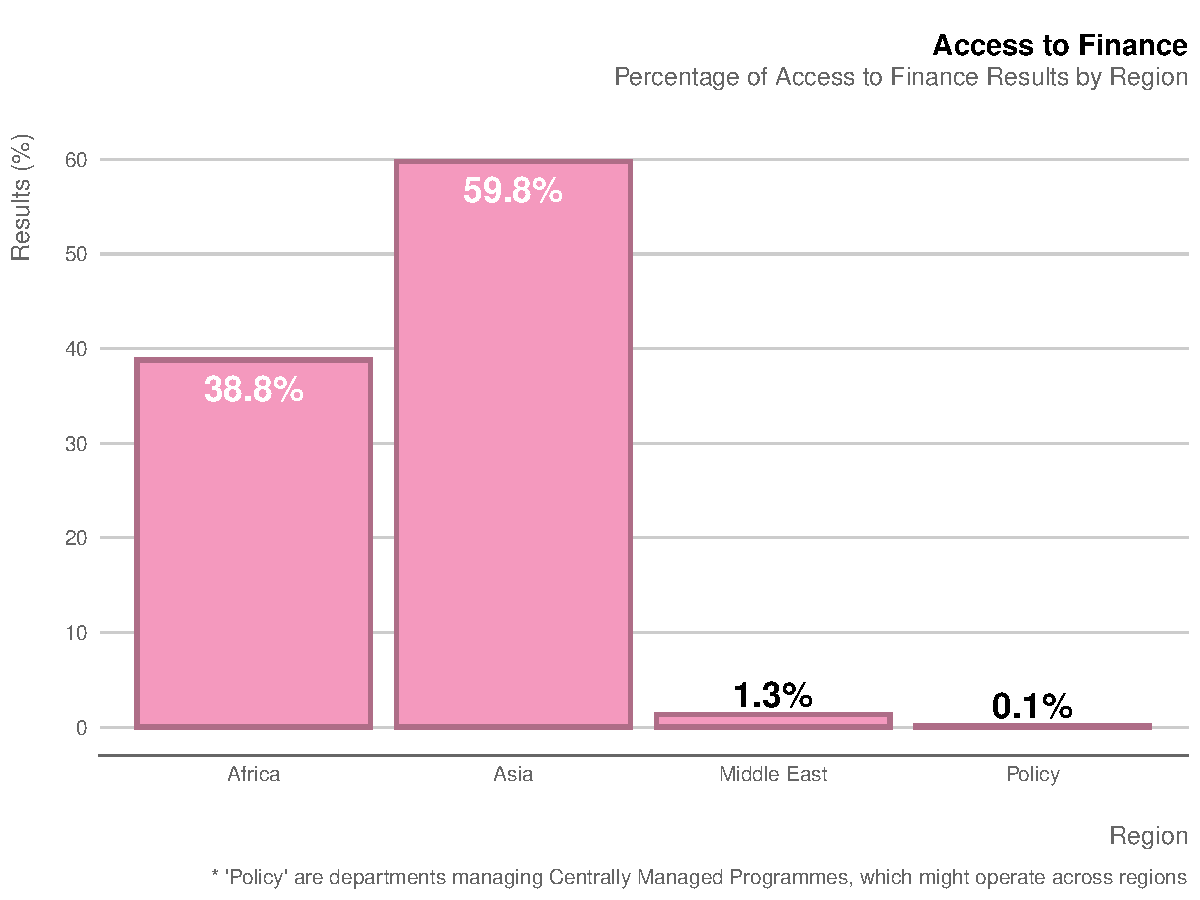
\includegraphics[width=0.8\textwidth]{../figs/a2f_region_plot} \hfill
	\caption{Percentage of Access to Finance results by region.}
	\label{fig:a2f_region_plot}
\end{figure}

\section{Context}
DFID’s Economic Development Strategy aims to `improve access to finance for both poor women and men,
helping them to generate and protect their own wealth.' %
This includes supporting improved access to financial services such as secure savings, money transfer, insurance and affordable loans. %

Access to financial services is expected to enhance the welfare of poor households by helping them to
smooth consumption, invest in enterprise, save and become more resilient to all kinds of economic, social
and environmental shocks, send and receive remittances (potentially with less associated costs) and
access credit if and when needed e.g. through access to affordable mortgages. %

DFID support in this area ensures that basic financial services are provided, there is facilitation of businesses growth and job creation, and that people are given support to better manage their own lives and help to escape poverty. %

\newpage

 \chapter{CDC Development Impact Grid Score}

\section*{A rolling weighted average (by investment \pounds) of the Development Impact Grid scores across all of CDC's investments that have reached financial close during the preceding three calendar years.}


\thispagestyle{empty}


\section{Results}

The weighted average Development Impact (DI) score for all CDC investments made from 2017-2019 is \textbf{2.94}. %

\section{Context}

CDC is an investment company, wholly owned by DFID. It invests in businesses in
Africa and South Asia to create jobs, catalyse private sector investment and build
markets in the world's poorest countries. \\%

The Development Impact Grid incentivises CDC to make investments in harder geographies and in sectors which have the highest propensity to create jobs. %
It is a tool to measure the shift in CDC's investment portfolio to more impactful investments. \\%

Each investment by CDC is given a Development Impact Grid score between 1 and 4. %
A score of 1 indicates lower investment difficulty and a lower propensity of the sector to generate employment. %
Conversely a score of 4 indicates higher investment difficulty, but the propensity of the sector to generate employment may be low, medium or high. %
This indicator measures the rolling, weighted (by investment \pounds) average of the Development Impact Grid scores across all of CDC's investments that have reached financial close during the preceding three calendar years. \\%

\newpage

 \chapter{Climate Finance}

\section*{Spend on building the resilience of poor people to the impacts of climate change and investing in low carbon development to avoid or reduce harmful greenhouse gases.}


\thispagestyle{empty}



\section{Results}
From 2016/17 to 2019/20, DFID spent \textbf{\pounds 2.9 billion} on building the resilience of poor people to the impacts of climate change and investing in low carbon development to avoid or prevent harmful greenhouse gases. %
This indicator contributes to the UK commitment to spend  \pounds  5.8 billion over five years on tackling climate change, of which DFID intends to spend \pounds3.6 billion. \\ %

\pounds 2.6 billion of DFID's spend on climate from 2016/17 to 2019/20 was through bilateral programmes by DFID's network of country offices, or by teams based in the UK whose programmes often operate across a range of countries. %
These programmes tackle climate change either as their main objective or alongside other development objectives such as economic development. \\ %

DFID, alongside the Department for Business, Energy and Industrial Strategy (BEIS) and the Department for Environment, Food and Rural Affairs (Defra), makes core contributions to specific multilateral organisations that tackle climate change, such as the Green Climate Fund and the Global Environment Facility. %
These organisations have greater reach across a broader range of countries and work with other donors to scale up climate finance faster and more effectively. %
DFID contributed \pounds 0.3 billion to climate multilaterals from 2016/17 to 2019/20. %

\begin{figure}[htbp]
  \centering
\begin{knitrout}
\definecolor{shadecolor}{rgb}{0.969, 0.969, 0.969}\color{fgcolor}
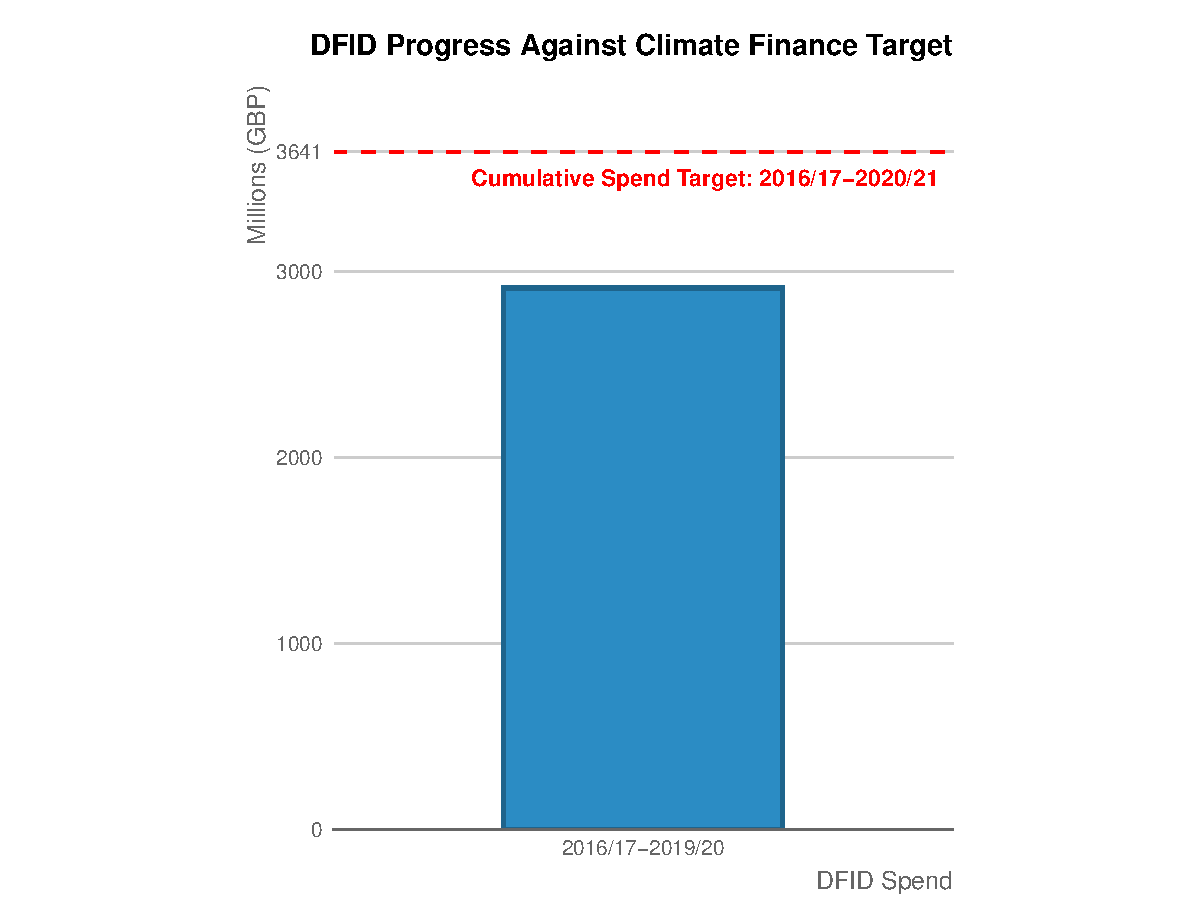
\includegraphics[width=0.8\textwidth]{figs/climate_spend_plot-1} 

\end{knitrout}
  \caption{DFID spend on climate finance from 2016/17 to 2019/2020 set against the cumulative spend target up to 2020/21 of \pounds 3,641 Million.}
  \label{fig:climate_spend_plot}
\end{figure}


\section{Context}

The World Bank estimates that an additional 100 million people could be in poverty by 2030 if climate change is not addressed. %
DFID recognises that poverty reduction and climate change are intrinsically linked and that action to tackle climate change must be embedded in DFID's work - in its engagement with partner countries, other donors and international organisations, and across its development portfolio - in order to drive sustainable decision-making in developing countries. \\%

The UK's International Climate Finance (ICF) aims to encourage transformational change in country resilience to climate change and disaster risk management, in sustainable management of natural resources such as forests, land and water and in access to clean energy and low carbon infrastructure. %
Alongside other developed countries, the UK has committed to jointly mobilise \$100 billion per year in climate finance to developing countries from public and private sources. %
DFID works jointly with BEIS and Defra on delivering this commitment using the UK aid budget. %

\subsection{Programmes using DFID Climate Finance}
Over 200 programmes contributed to DFID's climate finance spend during 2016/17-2019/20, using a range of instruments and covering a large number of sectors. %
Illustrative examples of this programming are noted below. \\%

DFID partnered with Germany to fund the Global Risk Financing Facility, which provides finance to support governments to use risk financing instruments, like insurance, to access more rapid finance in emergencies and to strengthen preparedness of local systems for disaster response and recovery. %
DFID also provided direct cash transfers to approximately 24,000 households living in arid and semi-arid areas of Kenya and has contributed to building a shock responsive system that now enables up to 374,000 households to be reached with cash in times of extreme drought emergencies. \\%

The Results Based Financing (RBF) for Low Carbon Energy Access programme has, since 2012 delivered energy access to at least 5.7 million people. %
A particularly successful model has been the Off-Grid Appliances RBF which has involved a bulk procurement incentive to distributors to deliver quality tested super- efficient off grid appliances like fridges, solar water pumps, and fans. This has led to the sale of over 250,000 efficient appliances in East Africa and Bangladesh through over 100 distributors to date. %
DFID support has enhanced Nepal's technical and negotiating capacity with a mix of home-grown expertise and international specialists to unlock investment in its hydro power export potential. %
Nepal is now set to double its current generation capacity, with a major \$1.2bn 900MW hydro power project currently under construction. \\%

DFID aims to drive a transformation towards sustainable management of these natural resources and protect the livelihoods of those who depend on them. %
DFID funding to the Forests Governance, Markets and Climate programme informed revision, in December 2019, of forest law in China to ban buying, transporting or processing illegally sourced timber, a major milestone in tackling illegal deforestation. \\%

In 2019, the UK (represented by DFID) held the developed country chair of the Green Climate Fund (GCF) Board. %
During this period, 32 projects worth US\$3.6 billion of GCF funding were approved by the GCF Board, including a solar rural electrification programme in Mali, directly benefiting 284,000 people and a clean cooking programme in Kenya and Senegal, directly benefiting over 11 million people. %
The GCF also completed its first replenishment, totalling US\$9.8 billion from 28 donors over the next four years, with the UK being the largest donor having doubled its contribution to \pounds 1.44 billion, funded by DFID and BEIS. \\%

Further information on UK International Climate Finance (ICF), including case studies, can be found on \href{https://www.gov.uk/guidance/international-climate-finance#our-portfolio-across-the-world}{GOV.UK} along with the \href{https://www.gov.uk/government/publications/uk-climate-finance-results}{latest UK Climate Finance Results}. %


\newpage

 \chapter{Development Capital Investment Levels}

\section*{Levels of development capital investment --- cumulative GBP from 2015-16 onwards.}

\thispagestyle{empty}

\bigskip
\bigskip

\section{Results}
DFID invested �3,039 million in Development Capital (DevCap) to create more and better inclusive jobs that benefit people across society, including women.

\section{Context}

The finance needed to achieve the Sustainable Development Goals is estimated at approximately \$ 2.5 trillion every year but current investment levels are less than half of that. %
DFID uses a range of instruments to finance progress against development objectives, but public resources alone will not be sufficient to address such high financing needs in developing countries. %
They will need to be used increasingly as a catalyst to attract private finance, especially to sectors that can transform developing
economies. %
However, investors often see markets in the poorest countries as too risky. %
To help fill this financing gap DFID plan to increase the use of instruments such as DevCap. %
This will then spur other private finance to follow over time, once DFID investment has created the demonstration effect necessary to attract investors. %

\newpage

 \chapter{Education}

\section*{Number of children supported to gain a decent education.}
% make sure numbers and header don't appear

\thispagestyle{empty}


\section{Results}
Between 2015 and 2020 DFID supported at least \textbf{15.6 million} children to gain a decent education. %

This is the equivalent number of children fully educated by DFID. %
All DFID education programmes include a focus on quality of education, so all children counted are being helped to gain a decent education. %

\begin{figure}[htbp]
  \centering
  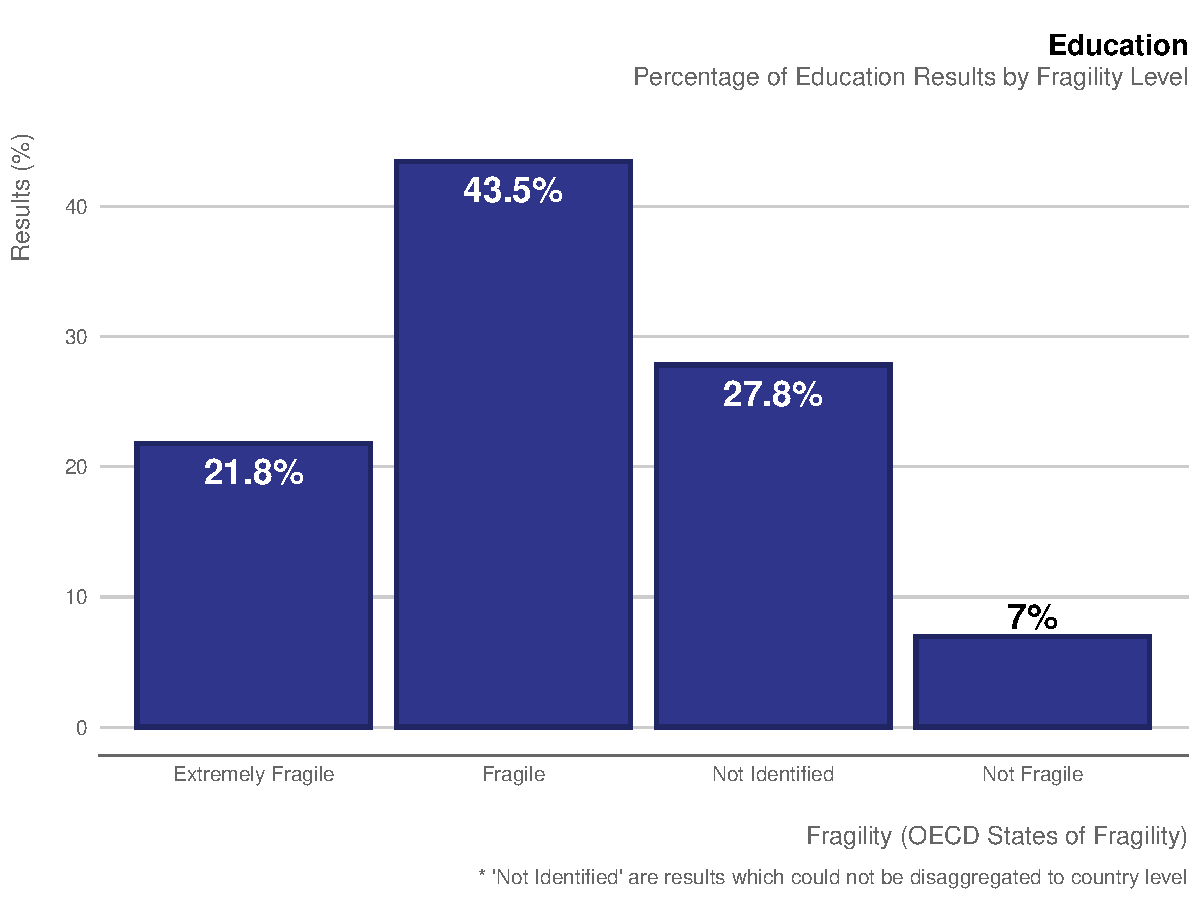
\includegraphics[width=0.8\textwidth]{../figs/education_fragility_plot} \hfill
  \caption{Percentage of Education results by fragility level.}
  \label{fig:edu_fragility_plot}
\end{figure}

From 2015 to 2020, the largest number of children supported by DFID education programmes were in Africa, with 5.6 million children supported (including 1.2 million in Ethiopia). %
DFID supported 5.3 million children in Asia (including 1.8 million in Bangladesh, and 2.1 million in Pakistan), and 0.8 million children in the Middle East. %
A further 4.6 million children were supported via centrally managed programmes and multilateral organisations. %

\begin{figure}[htbp]
	\centering
	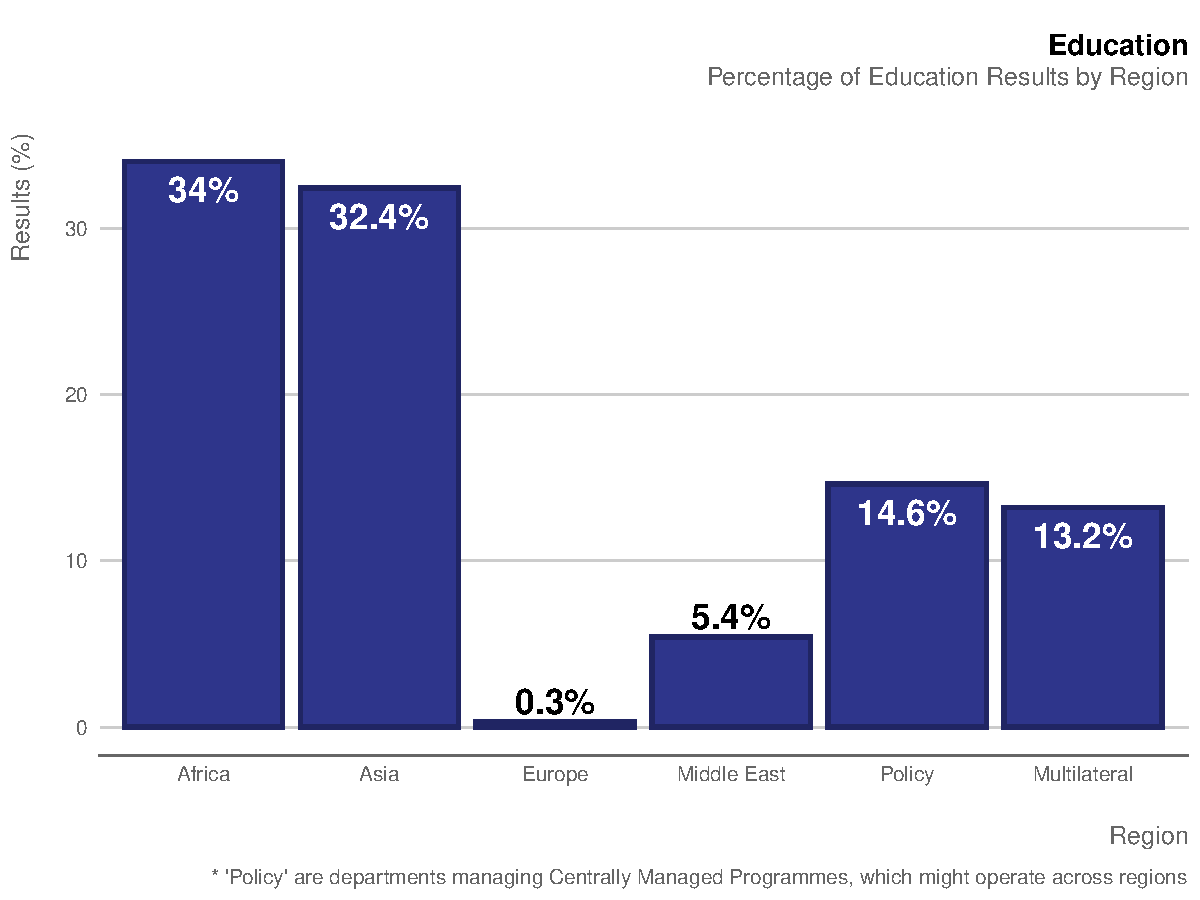
\includegraphics[width=0.8\textwidth]{../figs/education_region_plot} \hfill
	\caption{Percentage of Education results by region.}
	\label{fig:edu_region_plot}
\end{figure}

DFID uses the OECD list of fragile states, which is used to ensure our resources are focussed on fragile states. %
Most of the children supported by DFID's education programmes live in fragile states (10.8 million children), including 3.6 million living in extremely fragile states. %

Of the results that can currently be disaggregated by gender from 2015 to 2020 DFID education programs supported 8.1 million girls (over 50\% of the results). %
DFID is continuously working with our partners to improve collection of disaggregated data.
Over 95\% of our results are disaggregated by gender in part due to improvments in calculating children reached by multilateral organisations. %


\section{Context}

Education has wide ranging social, health and economic benefits. %
The latest evidence suggests:
\begin{itemize}
\item Each additional year of schooling typically results in a 10\% boost in earnings, with larger increases for women.\footnote{Montenegro, C. and Patrinos, H. (2014). Comparable Estimates of Returns to Schooling Around the World. Policy Research Working Paper. Washington DC: World Bank. Available from: \href{http://documents.worldbank.org/curated/en/830831468147839247/pdf/WPS7020.pdf}{http://documents.worldbank.org/curated/en/830831468147839247/pdf/WPS7020.pdf} [Accessed 26 January 2018]}
\item Educated women have a better understanding of healthy behaviour and are
more empowered to act on that knowledge. They have fewer children,
speeding the demographic transition, and their children are healthier and
more educated.\footnote{The International Commission on Financing Global Education Opportunity. (2016). The Learning Generation: Investing in Education for a Changing World. New York: The International Commission on Financing Global Education Opportunity. Available from: \href{http://report.educationcommission.org/downloads/}{http://report.educationcommission.org/downloads/} [Accessed 26 January 2018]}
\item Spending an additional year in secondary school can lower the risk of HIV
infection among students by around a third a decade later.\footnote{De Neve, J., Fink, G., Subramanian, S. V., Moyo, S., and Bor, J. (2015). Length of Secondary Schooling and Risk of HIV Infection in Botswana: Evidence From a Natural Experiment. The Lancet, 3: e470-477. Available from: \href{http://www.thelancet.com/pdfs/journals/langlo/PIIS2214-109X(15)00087-X.pdf}{http://www.thelancet.com/pdfs/journals/langlo/PIIS2214-109X(15)00087-X.pdf} [Accessed 26 January 2018]}
\end{itemize}

Developing countries have expanded schooling at an impressive rate in recent
decades. %
The average adult in 2010 had completed seven years of school, compared to only two in 1950. \footnote{World Bank. (2018). Learning to Realize Education’s Promise. World Development Report. Washington DC: World Bank. Available from: \href{http://www.worldbank.org/en/publication/wdr2018}{http://www.worldbank.org/en/publication/wdr2018} [Accessed 26 January 2018]}
Most children are now able to access education. %
Globally, over 97\% of children are expected to attend school at some time in their
lives. \footnote{\href{http://uis.unesco.org/sites/default/files/documents/reducing-global-poverty-through-universal-primary-secondary-education.pdf}{http://uis.unesco.org/sites/default/files/documents/reducing-global-poverty-through-universal-primary-secondary-education.pdf}}

Yet, many children are in school but failing to learn the basics: over half of all primary school aged children worldwide (387 million) are not on track to complete primary school or able to read well. \footnote{UIS factsheet No 46. \href{http://uis.unesco.org/sites/default/files/documents/fs46-more-than-halfchildren-not-learning-en-2017.pdf}{http://uis.unesco.org/sites/default/files/documents/fs46-more-than-halfchildren-not-learning-en-2017.pdf}}
This problem is particularly pronounced in subSaharan Africa and Central and South Asia, where nearly 85\% of primary aged children are not learning the basics. %

There are still 63 million of the most marginalised children out of primary school
(91\% of primary aged children globally) and a further 200 million out of secondary
school. %
Nearly a quarter of children with disabilities in developing countries are
estimated to never attend school\footnote{\href{http://uis.unesco.org/sites/default/files/documents/ip49-education-disability-2018-en.pdf}{http://uis.unesco.org/sites/default/files/documents/ip49-education-disability-2018-en.pdf}}; and children in conflict-affected countries are 1/3
less likely to complete primary school than those not affected by conflict.\footnote{The International Commission on Financing Global Education Opportunity. (2016). The Learning Generation: Investing in Education for a Changing World. New York: The International Commission on Financing Global Education Opportunity. Available from: \href{http://report.educationcommission.org/downloads/}{http://report.educationcommission.org/downloads/} [Accessed 26 January 2018].}


\newpage

 \chapter{Energy}

\section*{Level of clean energy capacity (megawatts) installed as a result of International Climate Finance (ICF) support.}

\thispagestyle{empty}



\section{Results}

From 2015/16 to 2019/20 DFID installed \textbf{
771
} of clean energy capacity (Table \ref{tab:energy}). %

\begin{figure}[htbp]
	\centering
\begin{knitrout}
\definecolor{shadecolor}{rgb}{0.969, 0.969, 0.969}\color{fgcolor}
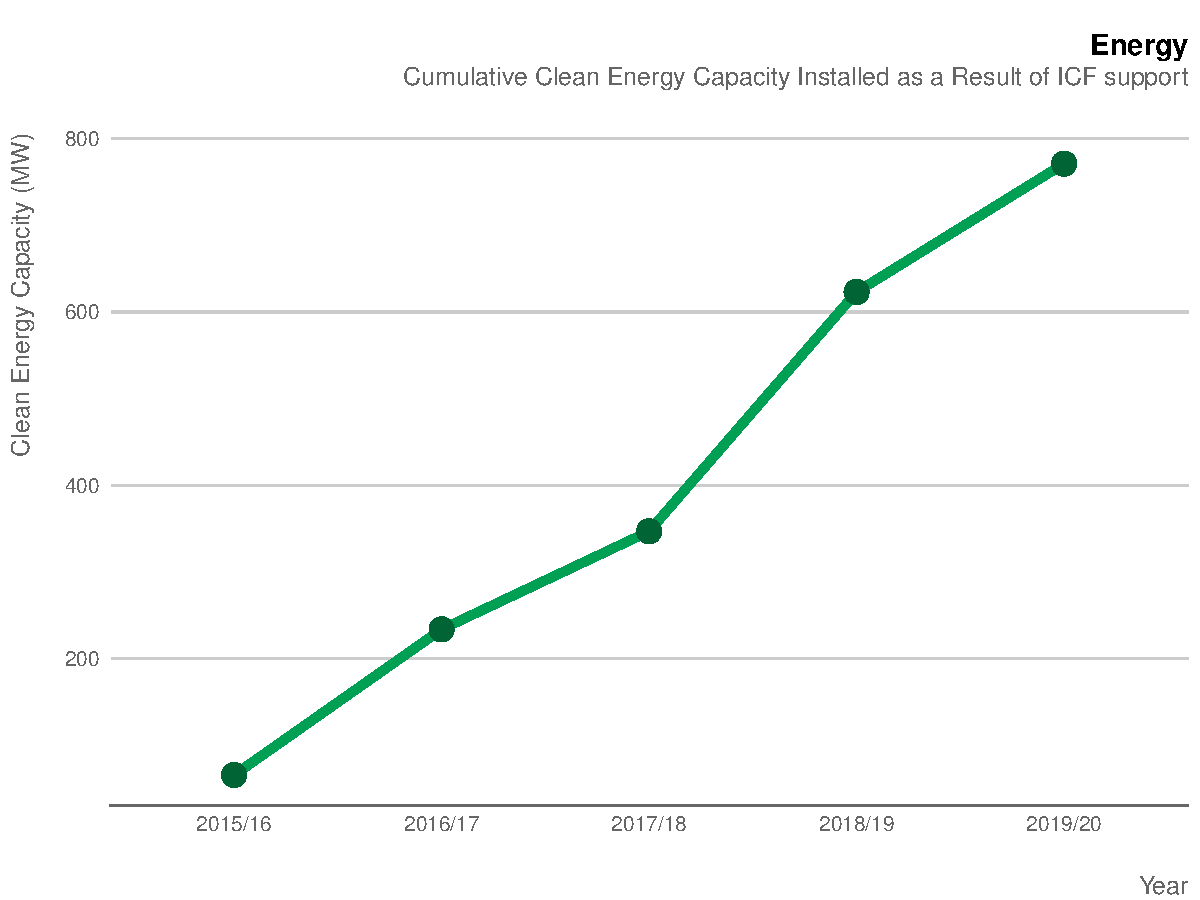
\includegraphics[width=0.8\textwidth]{figs/energy_cumulative_plot-1} 

\end{knitrout}
	%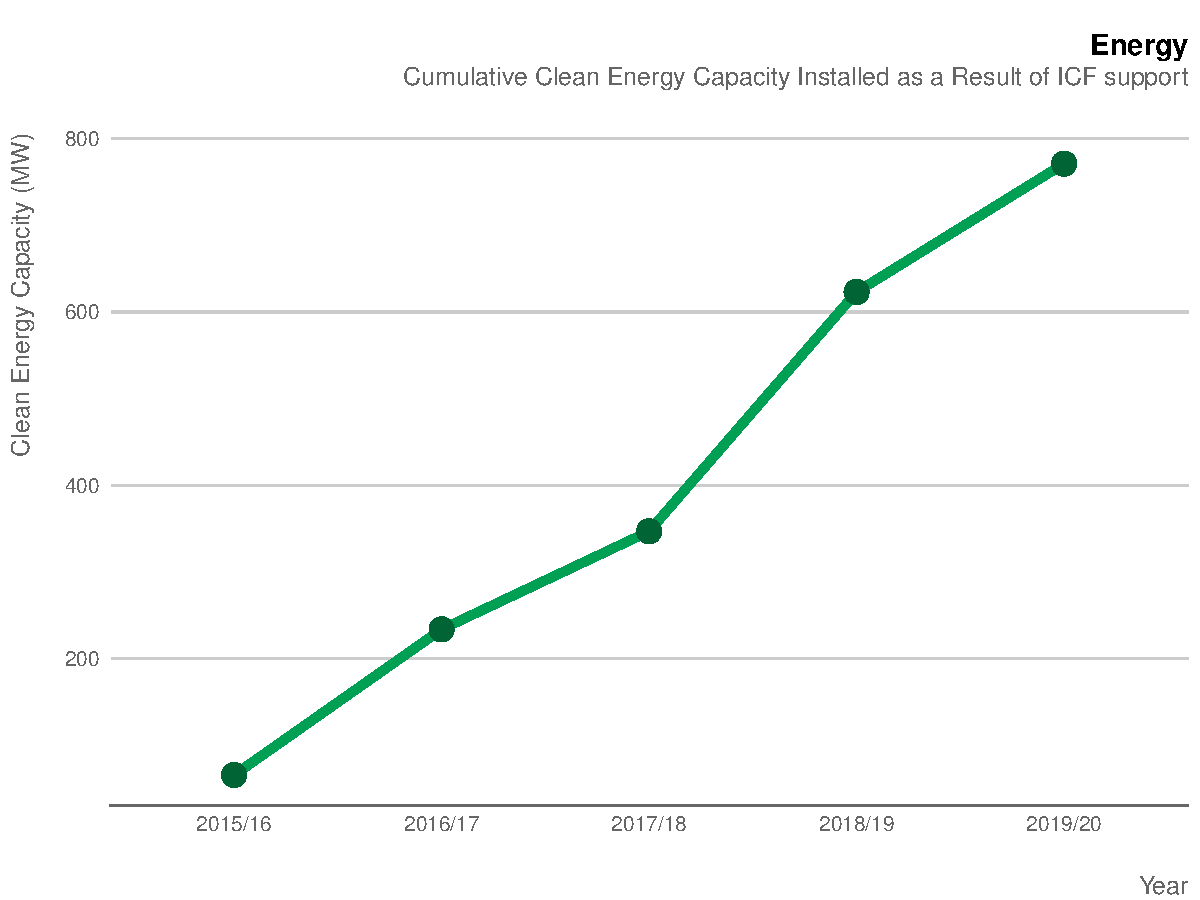
\includegraphics[width=0.7\textwidth]{../figs/energy_cumulative_plot} \hfill
	\caption{Line plot of cumulative clean energy capacity installed (in megawatts) from 2015/16 to 2019/20.}
	\label{fig:energy_cumulative_plot}
\end{figure}

When new information becomes available, historic estimates are updated during each annual results reporting round to reflect the best available information on programme achievements. %
As a result, several corrections to past years' data have been made this year. %
A number of programmes, which DFID has supported for multiple years, have reported results for the first time leading to an increase in historic results. %
Simultaneously, corrections were made to results estimates from the Clean Technology Fund (CTF), following a review by government analysts and the Climate Investment Fund's (CIFs) audit unit.  %
Corrections have been made where it was discovered that either results were being taken from the wrong source, data were inputted incorrectly, or inappropriate adjustments for over/under reporting had been made. %
These errors are difficult pick up during the quality assurance process since the CIFs rely on implementing partners to report project data accurately in the first instance. %

% Need to convert to xtable
\begin{table}[htbp]
	\centering
  \caption{Cumulative Totals of MW Clean Energy Capacity Installed (ICF KPI 7)}\label{tab:energy}
	\begin{tabular}{rrrrr}
		\toprule
		\multicolumn{1}{c}{\textbf{2015/16}}&\multicolumn{1}{c}{\textbf{2016/17}}&\multicolumn{1}{c}{\textbf{2017/18}}&\multicolumn{1}{c}{\textbf{2018/19}}&\multicolumn{1}{c}{\textbf{2019/20}} \\ \hline
		\rule{0pt}{10pt}66 	  &      234 	&        347 	   &     623 	  &        771 \\ \bottomrule
	\end{tabular}
\end{table}

\section{Context}

This indicator measures clean energy capacity installed as a result of DFID
programming. %

Access to energy is a constraint to inclusive economic growth and job creation across all of DFID's focus countries. %
Population growth is also pushing up energy demand; investments in electricity generation, transmission and distribution and connections have failed to keep pace. %
In our economic development strategy we made clear we will adopt a `climate smart' approach across our economic development work --- including through sustainable energy. %
We are working to help meet businesses' rising energy needs; to ensure affordable energy access for the poor; and to enhance environmental sustainability in energy use. %


\newpage

 \chapter{Family Planning}

\section*{Total Users: Number of women and girls using modern methods of family planning through DFID support.}

\section*{Additional Users: Number of additional women using modern methods of family planning through DFID support.}


\thispagestyle{empty}


\section{Results}

Between April 2015 and March 2020, DFID reached \textbf{
an average of 25.3 million
} \textbf{total} women and girls with modern methods of family planning per year\footnote{These figures are estimated using the Guttmacher publication (\href{https://www.guttmacher.org/report/adding-it-up-investing-in-sexual-reproductive-health-2019-methodology}{Adding It Up: Investing in Sexual and Reproductive Health 2019}), which estimates the reduction in unintended pregnancies, unsafe abortions, maternal deaths and traumas of still births and newborn deaths if unmet needs for modern contraceptive services are fulfilled in developing countries. For example, Guttmacher estimates that if the 218 million women currently facing an unmet need for contraception in developing countries are provided with services, this would reduce unintended pregnancies from 111 million to 35 million (i.e. by 76 million). Thus, the proportionate reduction in unintended pregnancies compared to unmet need is 34.8\% (i.e. 76 million/218 million). Multiplying this proportion by DFID's total user result for 2019 of 25.4 million gives 8.8 million unintended pregnancies averted due to DFID's support.}. %

Between April 2019 and March 2020 alone, at least
25.4
million total women and girls were reached, preventing: 8.8 million unintended pregnancies; 2.9 million unsafe abortions; saving 8,100 women's lives; and preventing the trauma of 81,900 stillbirths and 48,300 new-born deaths. %

% not generated in chunk
\begin{figure}
	\centering
	\subfloat{{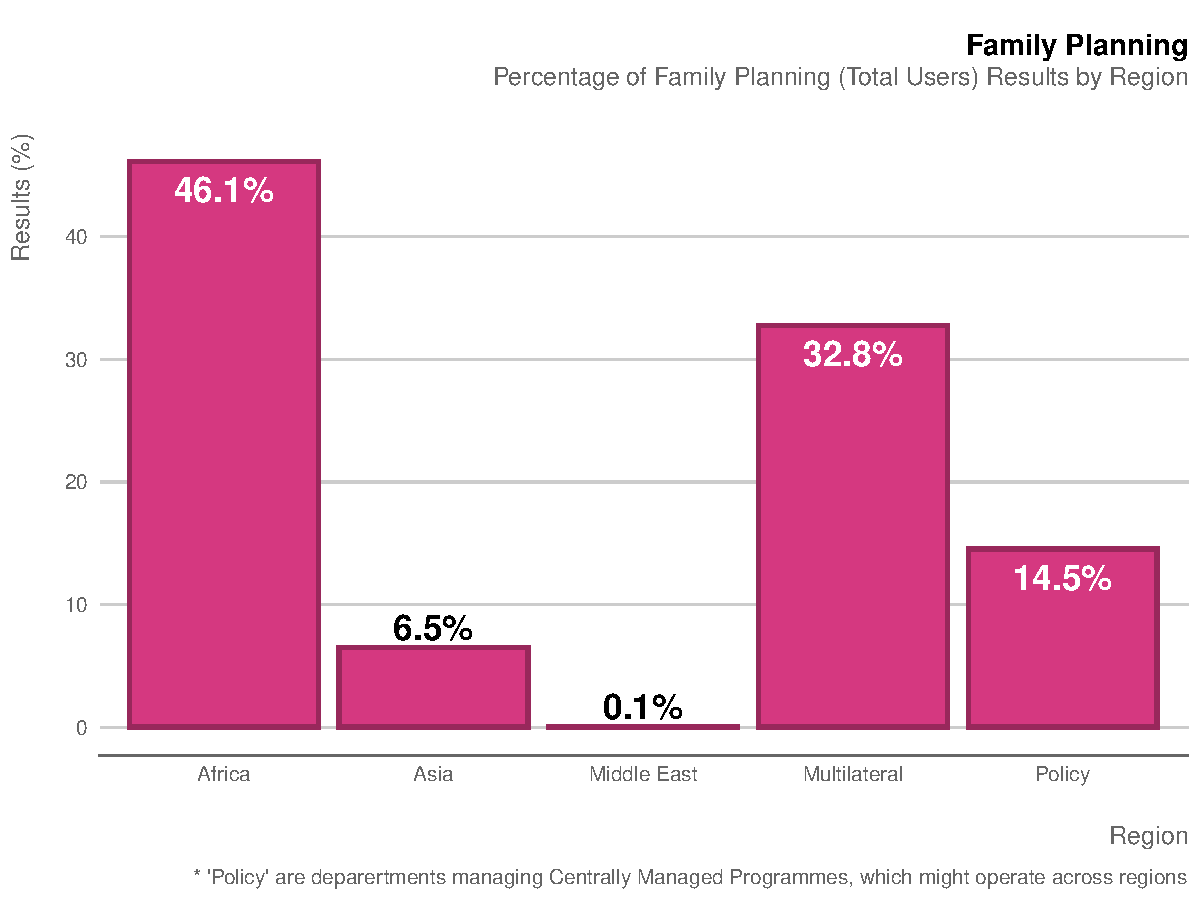
\includegraphics[width=0.8\textwidth]{../figs/fp_total_region_plot} }}%
	\qquad
	\subfloat{{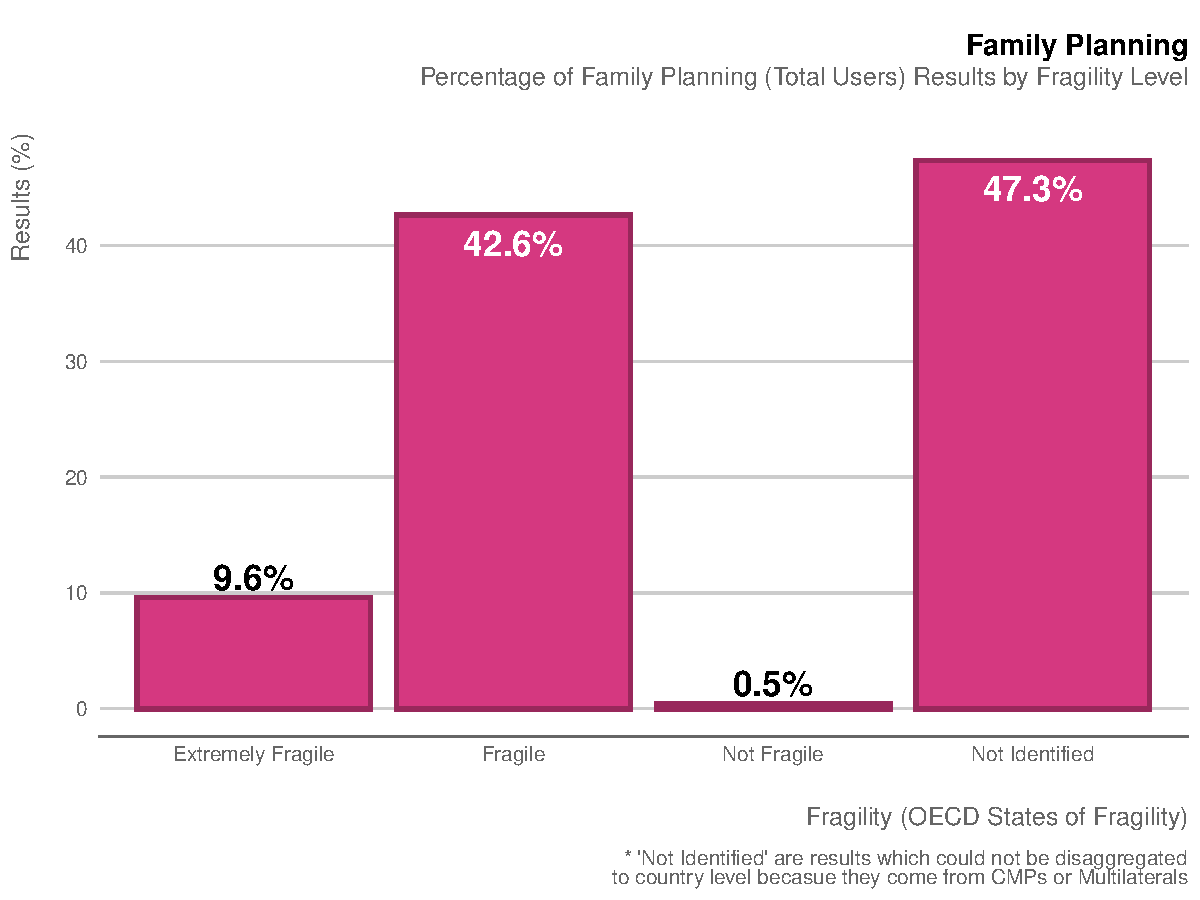
\includegraphics[width=0.8\textwidth]{../figs/fp_total_fragility_plot} }}%
	\caption{Percentage of Family Planning (Total) results by region and fragility level}%
	\label{fig:family_total}
\end{figure}

Between July 2012 and March 2020 DFID reached \textbf{
16.7 million
} \textbf{additional} women and girls with modern methods of family planning. %

Between April 2012 and March 2018, DFID spent an average of \pounds 193.6 million (approx.) on Family Planning every year. %

Between April 2017 and March 2018, DFID spent \pounds 241.5 million on Family Planning\footnote{\href{http://www.who.int/mediacentre/factsheets/fs351/en/}{http://www.who.int/mediacentre/factsheets/fs351/en/}}. %

% not generated in chunk
\begin{figure}
	\centering
	\subfloat{{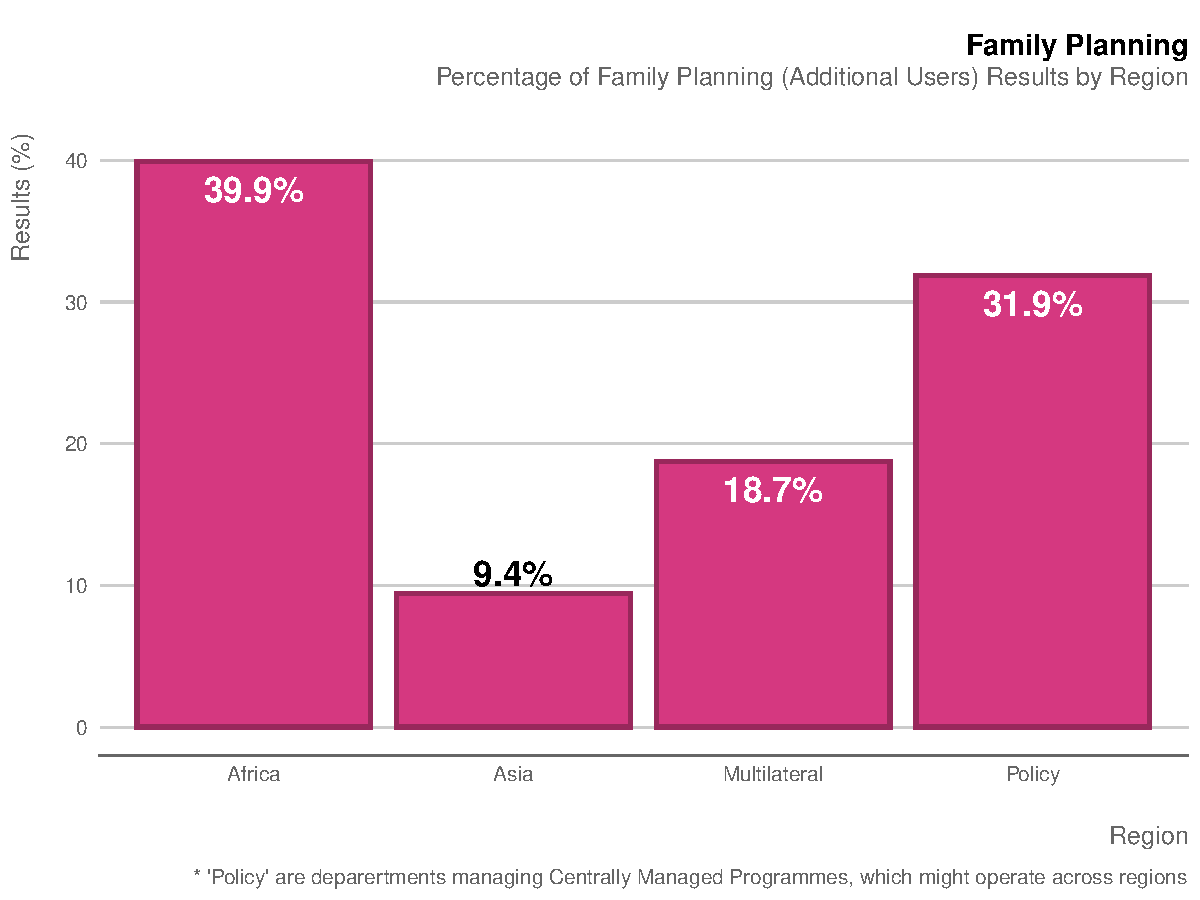
\includegraphics[width=0.8\textwidth]{../figs/fp_additional_region_plot} }}%
	\qquad
	\subfloat{{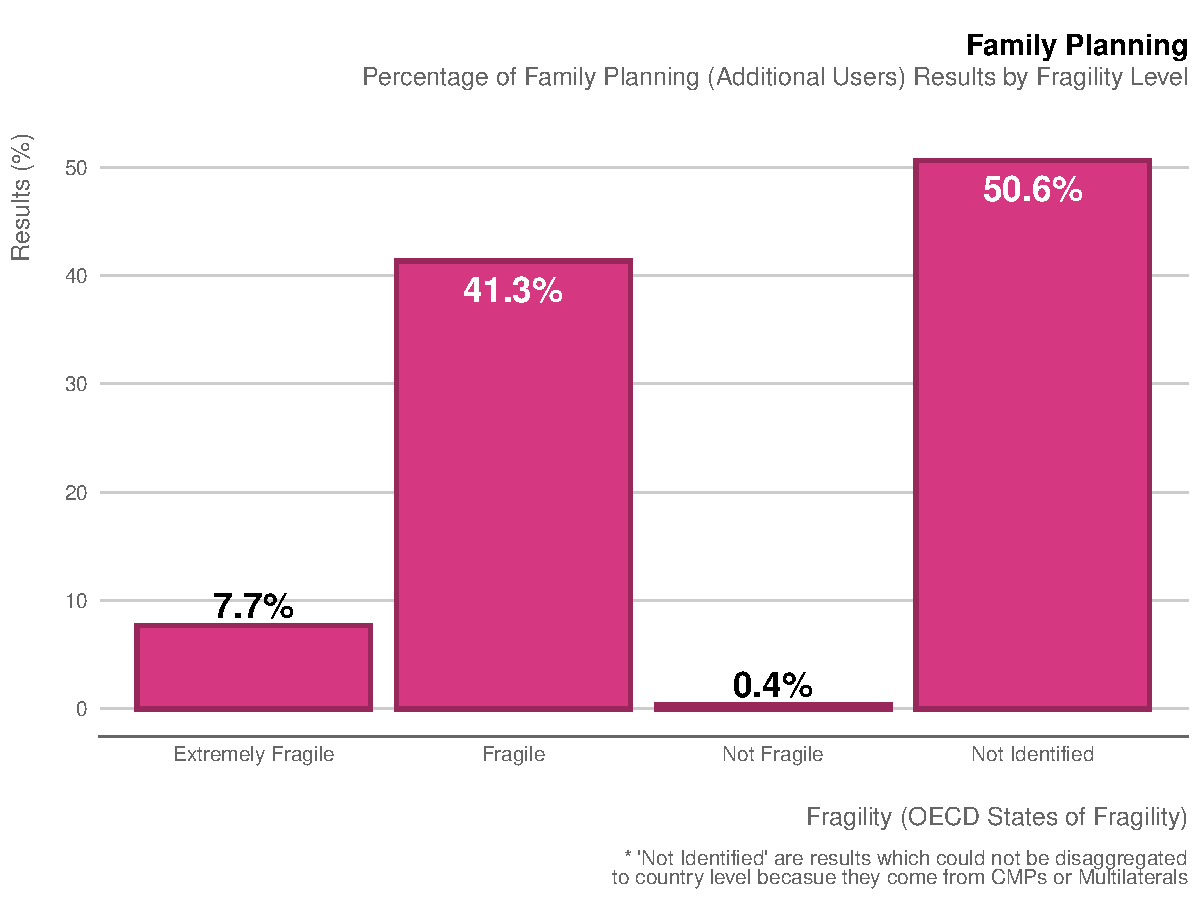
\includegraphics[width=0.8\textwidth]{../figs/fp_additional_fragility_plot} }}%
	\caption{Percentage of Family Planning (Additional) results by region and fragility level}
	\label{fig:family_additional}
\end{figure}


\section{Context}

Family planning is a major pillar of DFID's support to comprehensive Sexual and Reproductive Health and Rights. %
Family planning information, services and supplies enable women and girls to decide whether to have children, when and how many and to determine the spacing of pregnancies and is achieved via the use of modern contraceptive methods\footnote{\href{https://www.guttmacher.org/fact-sheet/adding-it-up-investing-in-sexual-reproductive-health}{https://www.guttmacher.org/fact-sheet/adding-it-up-investing-in-sexual-reproductive-health}}. %
This is fundamental to women and girl's empowerment, enabling them to have control over their lives helping to avoid early, multiple and frequently dangerous pregnancies and births, and instead complete their education, take up economic opportunities and fulfil their potential. %
There are an estimated 218 million women and girls, including 14 million adolescents in developing countries who want to time, space or prevent a pregnancy but are not using modern methods of family planning\footnote{\href{https://www.guttmacher.org/fact-sheet/adding-it-up-investing-in-sexual-reproductive-health-adolescents}{https://www.guttmacher.org/fact-sheet/adding-it-up-investing-in-sexual-reproductive-health-adolescents}}\footnote{\href{https://www.guttmacher.org/sites/default/files/report_downloads/adding-it-up-2019-report-appendix-tables.xlsx}{https://www.guttmacher.org/sites/default/files/report\_downloads/adding-it-up-2019-report-appendix-tables.xlsx}}. %
Unintended pregnancies and unsafe abortions would drop by about two-thirds each, and maternal deaths would reduce by more than one-fifth, if all women in developing countries wanting to avoid a pregnancy were to use modern contraceptives. %

Family Planning is one of the best investments in development. %
The Copenhagen Consensus estimated that every \$1 invested in meeting the unmet need for contraceptives yields in the long-term \$120 in accrued annual benefits (based on reduced infant and maternal mortality and long-term benefits from economic growth)\footnote{\href{http://www.familyplanning2020.org/sites/default/files/Data-Hub/ROI/FP2020_ROI_OnePager_FINAL.pdf}{http://www.familyplanning2020.org/sites/default/files/Data-Hub/ROI/FP2020\_ROI\_OnePager\_FINAL.pdf}}. %
Every dollar spent on contraceptive services beyond the current level would save \$3 in the cost of maternal, newborn and abortion care because use of contraceptives reduces the number of unintended pregnancies\footnote{\href{https://www.guttmacher.org/fact-sheet/adding-it-up-investing-in-sexual-reproductive-health}{https://www.guttmacher.org/fact-sheet/adding-it-up-investing-in-sexual-reproductive-health}}. %

The 2012 London Summit on Family Planning, hosted by the UK and the Bill and Melinda Gates Foundation, built on existing initiatives to put family planning higher on the global agenda, set international goals to enable women and girls to choose to use modern contraceptives and established the Family Planning 2020 (FP2020) partnership\footnote{\href{www.familyplanning2020.org}{www.familyplanning2020.org}}. %
The UK is a core convenor of this partnership, the second largest global bilateral donor on family planning, and co-funds the FP2020 Secretariat\footnote{\href{http://www.track20.org/pages/resources/FP2020_annual_reports.php}{http://www.track20.org/pages/resources/FP2020\_annual\_reports.php}}. %
In 2017, the UK co-hosted a follow-up Family Planning Summit with the Bill and Melinda Gates Foundation and UNFPA. %
The summit focused on innovation and tackling the barriers to progress. %
Over 50 countries, as well as civil society organisations, private sector partners and foundations made commitments to accelerate progress\footnote{\href{http://summit2017.familyplanning2020.org/}{http://summit2017.familyplanning2020.org/}}. %

The Department for International Development, UK (DFID) delivers family planning programmes in support of accelerating progress on voluntary family planning in developing countries and the UK's spend commitment. %
DFID funds a wide range of programmes in this area. %
Many support an integrated package of services for reproductive, maternal, newborn and child health through government facilities and the private sector. %
Some programmes provide contraceptives and other key commodities and others include strong aspects of community work to increase demand and change the social norms around accessing family planning. %
Results are tracked across all these different types of programmes using two indicators:
\begin{adjustwidth}{0.5cm}{}
\textbf{Total Users:} This indicator is defined as the number of women and girls who are currently using, or whose sexual partner is currently using at least one method of modern contraception through DFID's support. %
This indicator not only takes into account DFID's support to maintaining existing users of family planning and but also DFID's work to reach to new users of contraception in developing countries\footnote{This term refers to first-time users of contraception and/or users not recently using a method (e.g. a lapsed user)}. %

\medskip

\noindent\textbf{Additional Users:} Additional users are defined as the difference in total family planning users between years. Therefore, this indicator tracks DFID's support to expanding access to family planning in developing countries.%
\end{adjustwidth}


\newpage

 \chapter{Fragile and Conflicted Affected States}

\section*{Percentage of DFID's budget spent on fragile states and conflicted affected states.}

\bigskip
\bigskip

\thispagestyle{empty}


\section{Results}

In 2020, DFID adopted the OECD definition of fragile states. %
This list is regularly updated by the OECD and may result in the countries included within this indicator changing over time. %
Since this is a change from the list used previously (defined by DFID), the data is provided using both lists to demonstrate the imapct of the change. %
Differences between the previous DFID list, and the OECD list are presented in Table \ref{tab:fcas_fragstates}. %
There are 11 countries unique to the OECD list and 20 unique to the DFID list, reflecting the broader inclusion criteria of the previous DFID definition of fragile states. \\ %

\noindent\textbf{In 2018\footnotemark, according to the OECD list of fragile states and regions published in 2018, DFID spent 54 \% of its budget on fragile states.} \\ %

\footnotetext{Calculation of spend in fragile states requires breakdown of multilateral contributions by country, which are only available for final statistics on ODA in autumn each year. The next final statistics on ODA for 2019 will be published in autumn 2020, therefore, spend in fragile states for 2019 will be published in 2021.\label{fcas_note1}}

\noindent\textbf{In 2018\footref{fcas_note1}, according to the previous DFID list of fragile states and regions published in 2017, DFID spent 56 \% of its budget on fragile states and regions.} \\ %






\section{Context}
People who live in fragile and unstable places are more likely to remain in poverty. %
This input indicator demonstrates the priority DFID gives to tackling the causes of instability, insecurity and conflict. %

\begin{table}[htbp]
	\centering
	\caption{OECD States of Fragility 2018 Comparison to DFID 2017 List}\label{tab:fcas_fragstates} 
		\scriptsize
	\begin{tabular}{lcc}
		\toprule
		\multicolumn{1}{c}{\textbf{Country}}         & \textbf{OECD} (2018)               & \textbf{DFID} (2017)               \\ \hline
		\rule{0pt}{7pt}Afghanistan                             & \cellcolor[HTML]{E2EFD9}X & \cellcolor[HTML]{E2EFD9}X \\
		Algeria                                 &                           & \cellcolor[HTML]{FBE4D5}X \\
		Angola                                  & \cellcolor[HTML]{E2EFD9}X & \cellcolor[HTML]{E2EFD9}X \\
		Armenia                                 &                           & \cellcolor[HTML]{FBE4D5}X \\
		Azerbaijan                              &                           & \cellcolor[HTML]{FBE4D5}X \\
		Bangladesh                              & \cellcolor[HTML]{E2EFD9}X & \cellcolor[HTML]{E2EFD9}X \\
		Belarus                                 &                           & \cellcolor[HTML]{FBE4D5}X \\
		Benin                                   &                           & \cellcolor[HTML]{FBE4D5}X \\
		Burkina   Faso                          & \cellcolor[HTML]{FFF2CC}X &                           \\
		Burma                                   & \cellcolor[HTML]{E2EFD9}X & \cellcolor[HTML]{E2EFD9}X \\
		Burundi                                 & \cellcolor[HTML]{E2EFD9}X & \cellcolor[HTML]{E2EFD9}X \\
		Cameroon                                & \cellcolor[HTML]{E2EFD9}X & \cellcolor[HTML]{E2EFD9}X \\
		Central   African Republic              & \cellcolor[HTML]{E2EFD9}X & \cellcolor[HTML]{E2EFD9}X \\
		Chad                                    & \cellcolor[HTML]{E2EFD9}X & \cellcolor[HTML]{E2EFD9}X \\
		Colombia                                &                           & \cellcolor[HTML]{FBE4D5}X \\
		Comoros                                 & \cellcolor[HTML]{E2EFD9}X & \cellcolor[HTML]{E2EFD9}X \\
		Congo                                   & \cellcolor[HTML]{E2EFD9}X & \cellcolor[HTML]{E2EFD9}X \\
		Cote   d'Ivoire                         & \cellcolor[HTML]{FFF2CC}X & \cellcolor[HTML]{FFFFFF}  \\
		Democratic   People's Republic of Korea & \cellcolor[HTML]{E2EFD9}X & \cellcolor[HTML]{E2EFD9}X \\
		Democratic   Republic of the Congo      & \cellcolor[HTML]{E2EFD9}X & \cellcolor[HTML]{E2EFD9}X \\
		Djibouti                                & \cellcolor[HTML]{E2EFD9}X & \cellcolor[HTML]{E2EFD9}X \\
		Egypt                                   & \cellcolor[HTML]{E2EFD9}X & \cellcolor[HTML]{E2EFD9}X \\
		Equatorial   Guinea                     & \cellcolor[HTML]{FFF2CC}X &                           \\
		Eritrea                                 & \cellcolor[HTML]{E2EFD9}X & \cellcolor[HTML]{E2EFD9}X \\
		Eswatini                                & \cellcolor[HTML]{FFF2CC}X &                           \\
		Ethiopia                                & \cellcolor[HTML]{E2EFD9}X & \cellcolor[HTML]{E2EFD9}X \\
		Gambia                                  & \cellcolor[HTML]{E2EFD9}X & \cellcolor[HTML]{E2EFD9}X \\
		Guatemala                               & \cellcolor[HTML]{FFF2CC}X &                           \\
		Guinea                                  & \cellcolor[HTML]{E2EFD9}X & \cellcolor[HTML]{E2EFD9}X \\
		Guinea-Bissau                           & \cellcolor[HTML]{E2EFD9}X & \cellcolor[HTML]{E2EFD9}X \\
		Guyana                                  &                           & \cellcolor[HTML]{FBE4D5}X \\
		Haiti                                   & \cellcolor[HTML]{E2EFD9}X & \cellcolor[HTML]{E2EFD9}X \\
		Honduras                                & \cellcolor[HTML]{E2EFD9}X & \cellcolor[HTML]{E2EFD9}X \\
		Iran                                    & \cellcolor[HTML]{E2EFD9}X & \cellcolor[HTML]{E2EFD9}X \\
		Iraq                                    & \cellcolor[HTML]{E2EFD9}X & \cellcolor[HTML]{E2EFD9}X \\
		Jordan                                  &                           & \cellcolor[HTML]{FBE4D5}X \\
		Kenya                                   & \cellcolor[HTML]{E2EFD9}X & \cellcolor[HTML]{E2EFD9}X \\
		Kyrgyzstan                              &                           & \cellcolor[HTML]{FBE4D5}X \\
		Lao   People's Democratic Republic      & \cellcolor[HTML]{E2EFD9}X & \cellcolor[HTML]{E2EFD9}X \\ \bottomrule
	  \end{tabular}
	  \hspace{1em}
	  \begin{tabular}{lcc}
	  \toprule
		\multicolumn{1}{c}{\textbf{Country}}         & \textbf{OECD} (2018)               & \textbf{DFID} (2017)               \\ \hline
		\rule{0pt}{7pt}Lebanon                                 &                           & \cellcolor[HTML]{FBE4D5}X \\
		Liberia                                 & \cellcolor[HTML]{E2EFD9}X & \cellcolor[HTML]{E2EFD9}X \\
		Libya                                   & \cellcolor[HTML]{E2EFD9}X & \cellcolor[HTML]{E2EFD9}X \\
		Madagascar                              & \cellcolor[HTML]{E2EFD9}X & \cellcolor[HTML]{E2EFD9}X \\
		Malawi                                  & \cellcolor[HTML]{FFF2CC}X &                           \\
		Mali                                    & \cellcolor[HTML]{E2EFD9}X & \cellcolor[HTML]{E2EFD9}X \\
		Mauritania                              & \cellcolor[HTML]{E2EFD9}X & \cellcolor[HTML]{E2EFD9}X \\
		Middle   East, regional                 &                           & \cellcolor[HTML]{FBE4D5}X \\
		Moldova                                 &                           & \cellcolor[HTML]{FBE4D5}X \\
		Mozambique                              & \cellcolor[HTML]{FFF2CC}X &                           \\
		Nepal                                   & \cellcolor[HTML]{E2EFD9}X & \cellcolor[HTML]{E2EFD9}X \\
		Niger                                   & \cellcolor[HTML]{E2EFD9}X & \cellcolor[HTML]{E2EFD9}X \\
		Nigeria                                 & \cellcolor[HTML]{E2EFD9}X & \cellcolor[HTML]{E2EFD9}X \\
		North of   Sahara, regional             &                           & \cellcolor[HTML]{FBE4D5}X \\
		Pakistan                                & \cellcolor[HTML]{E2EFD9}X & \cellcolor[HTML]{E2EFD9}X \\
		Papua   New Guinea                      & \cellcolor[HTML]{FFF2CC}X &                           \\
		Rwanda                                  & \cellcolor[HTML]{E2EFD9}X & \cellcolor[HTML]{E2EFD9}X \\
		Sierra   Leone                          & \cellcolor[HTML]{FFF2CC}X &                           \\
		Solomon   Islands                       & \cellcolor[HTML]{FFF2CC}X &                           \\
		Somalia                                 & \cellcolor[HTML]{E2EFD9}X & \cellcolor[HTML]{E2EFD9}X \\
		South of   Sahara, regional             &                           & \cellcolor[HTML]{FBE4D5}X \\
		South   Sudan                           & \cellcolor[HTML]{E2EFD9}X & \cellcolor[HTML]{E2EFD9}X \\
		Sudan                                   & \cellcolor[HTML]{E2EFD9}X & \cellcolor[HTML]{E2EFD9}X \\
		Syrian   Arab Republic                  & \cellcolor[HTML]{E2EFD9}X & \cellcolor[HTML]{E2EFD9}X \\
		Tajikistan                              & \cellcolor[HTML]{E2EFD9}X & \cellcolor[HTML]{E2EFD9}X \\
		Tanzania                                & \cellcolor[HTML]{E2EFD9}X & \cellcolor[HTML]{E2EFD9}X \\
		Thailand                                &                           & \cellcolor[HTML]{FBE4D5}X \\
		Timor-Leste                             & \cellcolor[HTML]{FFF2CC}X &                           \\
		Tunisia                                 &                           & \cellcolor[HTML]{FBE4D5}X \\
		Turkey                                  &                           & \cellcolor[HTML]{FBE4D5}X \\
		Turkmenistan                            &                           & \cellcolor[HTML]{FBE4D5}X \\
		Uganda                                  & \cellcolor[HTML]{E2EFD9}X & \cellcolor[HTML]{E2EFD9}X \\
		Ukraine                                 &                           & \cellcolor[HTML]{FBE4D5}X \\
		Uzbekistan                              &                           & \cellcolor[HTML]{FBE4D5}X \\
		Venezuela                               & \cellcolor[HTML]{E2EFD9}X & \cellcolor[HTML]{E2EFD9}X \\
		West   Bank and Gaza Strip              & \cellcolor[HTML]{E2EFD9}X & \cellcolor[HTML]{E2EFD9}X \\
		Yemen                                   & \cellcolor[HTML]{E2EFD9}X & \cellcolor[HTML]{E2EFD9}X \\
		Zambia                                  & \cellcolor[HTML]{E2EFD9}X & \cellcolor[HTML]{E2EFD9}X \\
		Zimbabwe                                & \cellcolor[HTML]{E2EFD9}X & \cellcolor[HTML]{E2EFD9}X \\ \bottomrule
	\end{tabular}
\end{table}

\newpage

 \chapter{Humanitarian}

\section*{Number of people reached with humanitarian assistance (food aid, cash and voucher transfers) through DFID support.}
% make sure numbers and header don't appear

\thispagestyle{empty}

\section{Results}
From 2015 to March 2020 DFID reached \textbf{33.6 million} people with humanitarian assistance (food aid, cash and voucher transfers). %
This is a 1 million person (3\%) increase on the achieved reach from 2015 to March 2019, reported in July 2019. %

From 2015 to 2020 Africa was the largest beneficiary of DFID's humanitarian assistance programmes, with 18.4 million people reached --- approximately 5 out of every 10 people reached throughout the reporting period. %
The largest number of beneficiaries reached by DFID supported humanitarian programmes in a single African country was in Somalia (3.6 million people received humanitarian assistance). %

In the Middle East region DFID provided humanitarian assistance to 9 million beneficiaries, the majority of whom were located in Yemen (6.9 million people). %
More people were reached by DFID humanitarian programmes in Yemen, than in any other country. %

A further 4.2 million beneficiaries were from Asia. %
This includes 1.5 million people in Bangladesh and 1.6 million people in Pakistan. %

Finally, 500,000 people were assisted in Europe --- in the Ukraine and Turkey --- and 1.4 million people were reached via non-country specific and non-region specific programmes. %

\begin{figure}[htbp]
	\centering
	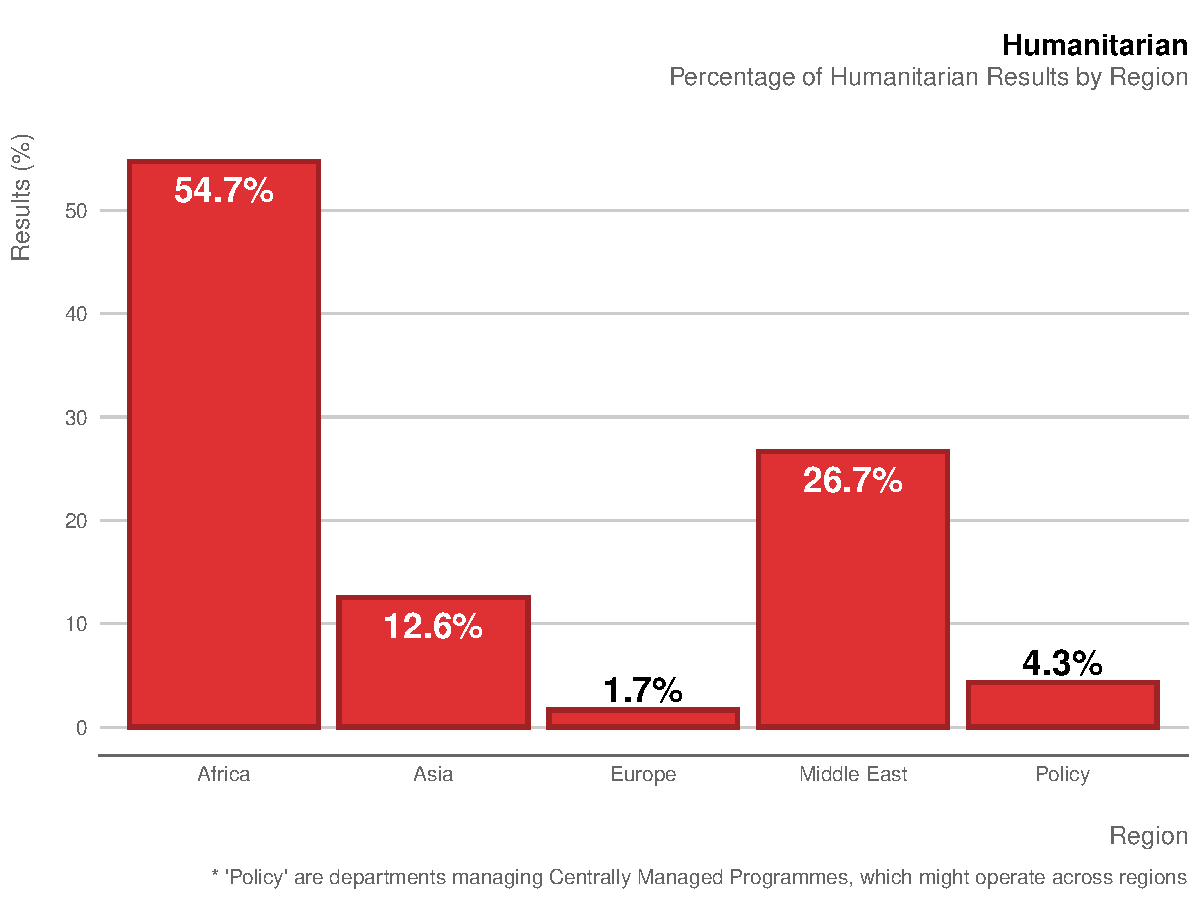
\includegraphics[width=0.8\textwidth]{../figs/human_region_plot} \hfill
	\caption{Percentage of Humanitarian results by region.}
	\label{fig:human_region_plot}
\end{figure}


Over 85\% (26.2 million beneficiaries) of the people reached by DFID supported humanitarian assistance live in fragile states (using the OECD States of Fragility definition). %
This includes 18.1 million beneficiaries living in Extremely Fragile states. %
A further 10.5\% (3.5 million beneficiaries) of DFID supported humanitarian assistance was delivered via non-country specific programmes and so it is not possible to assign a fragility level to these results. %


\begin{figure}[htbp]
	\centering
	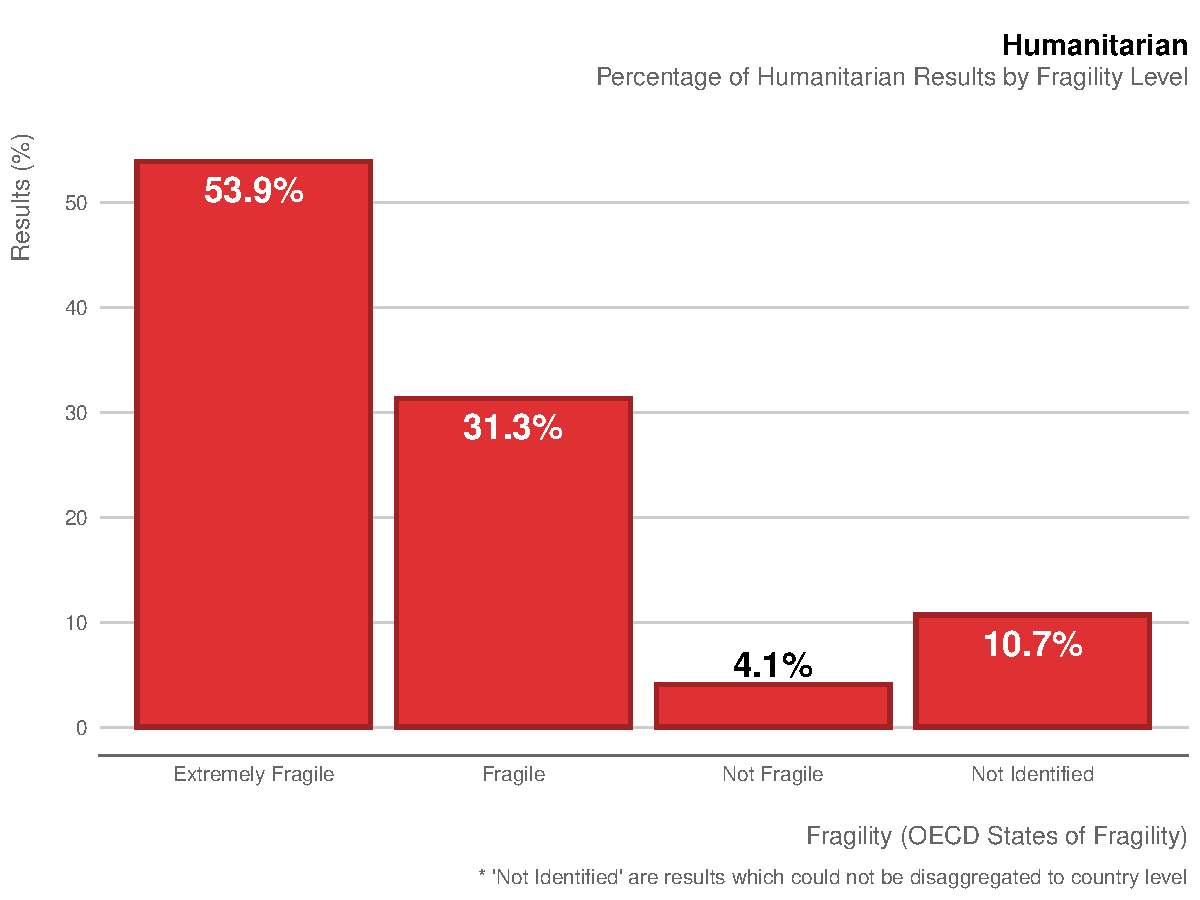
\includegraphics[width=0.8\textwidth]{../figs/human_fragility_plot} \hfill
	\caption{Percentage of Humanitarian results by fragility level.}
	\label{fig:human_fragility_plot}
\end{figure}


Of those reached by DFID humanitarian programmes from 2015 to March 2020, at least 40\% (13.7 million) were women and girls. %

DFID is continuously working with our existing partners towards improving collection of disaggregated data. %
In 2019/20, 76\% of our reported humanitarian results were disaggregated by gender. %
This is a 19 percentage point increase in data disaggregation by gender between the results reported in 2018/19 and 2019/20. %
There are considerable challenges with robust data collection in humanitarian contexts, particularly for people in greatest need. %
These are the generally the most unstable situations in which DFID supported programmes operate, where ongoing conflicts substantially increase the risks faced by those delivering emergency assistance and severely hinder access. %
DFID is collaborating with external partners to develop guidance, support and tools to facilitate data disaggregation but it should be recognised that DFID’s commitment to reach those people in greatest need means that data collection and reliable disaggregation in the most difficult humanitarian contexts will continue to be a considerable challenge. %


\section{Context}

Humanitarian aid provides essential material and support assistance to the world's most vulnerable people. %
It is usually short-term help provided in crisis situations to help victims of natural disasters, wars and famines. %
Humanitarian aid saves lives, relieves suffering and maintains human dignity. %
It differs from development aid, which seeks to address the underlying causes which may have led to a crisis or emergency. %

By its nature, humanitarian assistance is reactive to unplanned events, therefore, DFID has no specific targets for the amount of humanitarian assistance to be delivered. %
Instead, DFID focuses on delivering the best possible humanitarian assistance to people in need. %
By working with global and UK partners DFID endeavours to improve the UK's capacity to deliver timely, efficient, effective and equitable humanitarian aid, whenever and wherever it is needed. %
DFID recognises that this assistance should not just be delivered after an event when a crisis has been declared. %
Preventative action and early intervention are more effective --- delivering greater impact for a lower total investment, and preventing unnecessary suffering and loss of life in the early stages of a crisis. %
DFID is working to make responses more predictable and to help countries build resilience, prepare for crises, and manage the risk of crises through tools such as risk insurance. %

The United Nations Office for the Co-ordination of Humanitarian Affairs (OCHA) estimated that over 131.7 million people were in need of humanitarian aid in 2019\footnote{\href{https://www.unocha.org/sites/unocha/files/GHO-2020_v9.1.pdf}{https://www.unocha.org/sites/unocha/files/GHO-2020\_v9.1.pdf}}. %
The persisting drivers of increasing humanitarian need are conflict and protracted violence, while natural disasters, droughts, floods and hurricanes continue to create humanitarian need. %

In the 2019 period, 117.4 million people were targeted globally for humanitarian assistance. %
Fifty-four percent of the \$29.7bn financial requirement was met, leaving unmet requirements, or a funding gap, of \$13.7bn. %

In 2019, the UK provided \pounds 1.5bn in bi-lateral humanitarian aid, 9.9 \% of the total UK official development assistance (ODA) spend. %
This represents an increase of \pounds 208 million compared with 2018 and was partly driven by UK responses to humanitarian crises, for example in Yemen. %
These are provisional figures from Statistics in International Development; the full release in autumn 2020 will confirm final figures and DFID's share of total spend. %
In 2018, humanitarian assistance was the UK's second largest area of spend, after health, on sector specific ODA – \pounds 1,299 million (8.9 \% of UK ODA). %
DFID was responsible for around 99\% of the total UK ODA spend on humanitarian assistance. %

In addition to crisis or country specific spend the UK continues to be one of the largest contributors of core funding to the UN humanitarian agencies and the Red Cross movement, allowing these partners the flexibility to plan, invest in their capacity for timely and equitable humanitarian responses, and to direct resources to where the need is greatest. %
Recognising the UK's role as donors in delivering the vision of a more effective system in the face of unprecedented humanitarian needs worldwide, UK core funding was redesigned to create incentives for multilateral organisations to perform better. %
From 2018, 30\% of the UK's core funding to humanitarian agencies has been performance-based --- an approach known as ``Payment by Results'' (PbR) --- dependent on the delivery of vital reforms agreed at the World Humanitarian Summit in 2016, including the 'Grand Bargain'. %
In order to trigger full payment, agencies will have to demonstrate they have reformed their working practices in line with commitments to improve the effectiveness and efficiency of the international humanitarian system. %
The targets under PbR are ambitious and incentivise the UN and Red Cross movement to each work more collaboratively. %

In October 2017 the UK set out the new Humanitarian Reform Policy \footnote{\href{https://www.gov.uk/government/publications/uk-governments-humanitarian-reform-policy}{https://www.gov.uk/government/publications/uk-governments-humanitarian-reform-policy}} explaining both innovations and improvements in the UK's humanitarian response, and pushing for a more ambitious reform of the international humanitarian system. %
The UK will:
\begin{itemize}
\item Continue to protect people in crises: upholding humanitarian law and principles, uphold humanitarian law, and support our partners to do the same.
\item Deliver bigger, better, faster responses to rapid onset disasters when national systems are overwhelmed, as demonstrated in the Caribbean.
\item Invest in resilience and preparedness to respond, including using insurance and other risk-based finance to better manage risks from natural hazards.
\item Adopt a new long-term approach to protracted crises, including support to countries hosting long-term refugees to generate livelihoods, trading opportunities and invest in people’s future.
\item Challenge the international humanitarian system to hold itself to account for delivering better for people affected by crises, and ensuring the most vulnerable people in the world are appropriately protected from environmental and social hazards.
\item Ensure that response is delivered through organisations and mechanisms which offer best value for money, such as encouraging the use of multi-purpose cash transfers (where appropriate) which are faster, safer and more cost-effective than relief-in kind whilst providing additional support to local economies.
\end{itemize}

Single departmental plan results are attributed from DFID bi-lateral programmes and do not include the UK contribution to results attributed to UN or Red Cross agency central programmes where DFID is not a specific project partner. %


\newpage

 \chapter{Immunisations}

\section*{Number of lives saved by immunising children against killer diseases}

\bigskip
\bigskip

\thispagestyle{empty}


\section{Results}
From the start of 2015 until the end of 2018, DFID support immunised an estimated \textbf{74.3 million} children, saving \textbf{1.4 million} lives. %


\section{Context}

The World Health Organization (WHO) estimates that immunisation averts two to three million deaths every year and that, if global coverage improved, an additional one and a half million deaths could be averted. %
The WHO also estimated that 19.4 million infants lacked routine immunisations in 2018\footnotemark. \\%

\footnotetext{\href{https://www.who.int/en/news-room/fact-sheets/detail/immunization-coverage}{https://www.who.int/en/news-room/fact-sheets/detail/immunization-coverage}}

DFID provides funding to Gavi, the Vaccine Alliance with the intent of increasing immunisations. %
Gavi is an international organisation with the goal of increasing access to immunisations for children in low-income countries. %
All of DFID's results for this indicator come from Gavi results that are attributed to DFID based on the share of UK funding to Gavi. %

\newpage

 \chapter{Improving Tax Systems}

\section*{}


\thispagestyle{empty}


\section{Results}

In 2019, DFID invested \textbf{\pounds 29 million} on improving tax systems in developing countries. %


\section{Context}
Domestic tax reform in developing economies can mobilise additional public resources, crucial for sustainable development financing. %
DFID supports countries to raise and use their own revenues, in a way that enables sustainable and inclusive growth and reduces poverty. \\%

In 2015, at the Financing for Development Conference in Addis Ababa, the Secretary of State for International Development committed the UK to the \href{https://www.addistaxinitiative.net/}{Addis Tax Initiative}, a pledge to bolster tax for development work as a critical pathway to achieving the Sustainable Development Goals. %
As part of this, the UK committed to double the amount it spends on tax technical assistance and capacity building collectively with other donors (currently, there are 20 participating donors). \\%

The Single Departmental Plan monitors DFID-only spend on tax for development work. %
This is the figure at the top of this page. %
However, DFID works collaboratively with HM Treasury and HM Revenue and Customs on this work, the latter delivering peer-to-peer tax capacity building to support tax administration and policy reforms in developing countries. %
Therefore, as well as tracking DFID spend, we also track UK spend as a whole. %
This is the figure we report to the Addis Tax Initiative Secretariat, which is based in the International Tax Compact in Germany. \\%

The UK committed to double its spend on tax for development work, from a 2014 baseline of \pounds 25 million to \pounds 50 million in 2020. %

\newpage

 \chapter{Investment in the Multilateral System}



\section*{UK investment in the multilateral system (core multilateral ODA) compared with other Development Assistance Committee donors.}

\bigskip
\bigskip

\thispagestyle{empty}


\section{Results}

Provisional data indicates that in 2019 \pounds 5,061 million of UK ODA was delivered through core contributions to multilaterals (Table \ref{tab:multi_rank}). %
This was a 4.3 \% decrease (\pounds 228 million) compared to 2018. %
Between 2015 and 2018 the UK was consistently ranked top of DAC countries in its level of investment in the multilateral system. %


\begin{table}[htbp]
  \centering
  \caption{Core Contributions to Multilaterals and Rank Compared to DAC Members.}\label{tab:multi_rank}
  \begin{tabular}{lrc}
  \toprule
  \multicolumn{1}{c}{\textbf{Year}} & \multicolumn{1}{c}{\textbf{Core Multilateral ODA (\pounds) m}} & \multicolumn{1}{c}{\textbf{Rank}} \\ \hline
  \rule{0pt}{10pt}2015 & 4,473 & 1 \\
  2016 & 4,843 & 1 \\
  2017 & 5,256 & 1 \\
  2018 & 5,289 & 1 \\
  2019 & 5,061 & TBC\footnotemark \\
  \bottomrule
  \end{tabular}
\end{table}


\footnotetext{The value for 2019 is provisional and OECD data on donor rankings for 2019 is not yet available.\label{multi_note1}}


\section{Context}
The decrease in the volume of UK ODA delivered through core contributions to multilaterals between 2018 and 2019 was in part due to a smaller annual contribution to the International Development Association compared with 2018, in line with the planned payment schedule. %
Core contributions to multilaterals will fluctuate from year to year in part due to the payment schedules of the receiving multilateral organisation. %


\newpage

 \chapter{Jobs and Income}

\section*{Number of people supported to have raised incomes and better jobs  or livelihoods}

% make sure numbers and header don't appear
\thispagestyle{empty}


\section{Results}
From 2015/16 to 2019/20 DFID supported \textbf{5.1 million} people to raise their incomes or maintain/gain a better job or livelihood. %

\subsection{Results by gender}
Ninety-nine percent of results were broken down by gender. %
Of the 5.1 million people supported, 3.6 million were men and 1.5 million were women (figures do not sum due to rounding).

\subsection{Results by region}
See Figure \ref{fig:jobs_region_plot} for regional breakdown of results.  %


\begin{figure}[htbp]
	\centering
	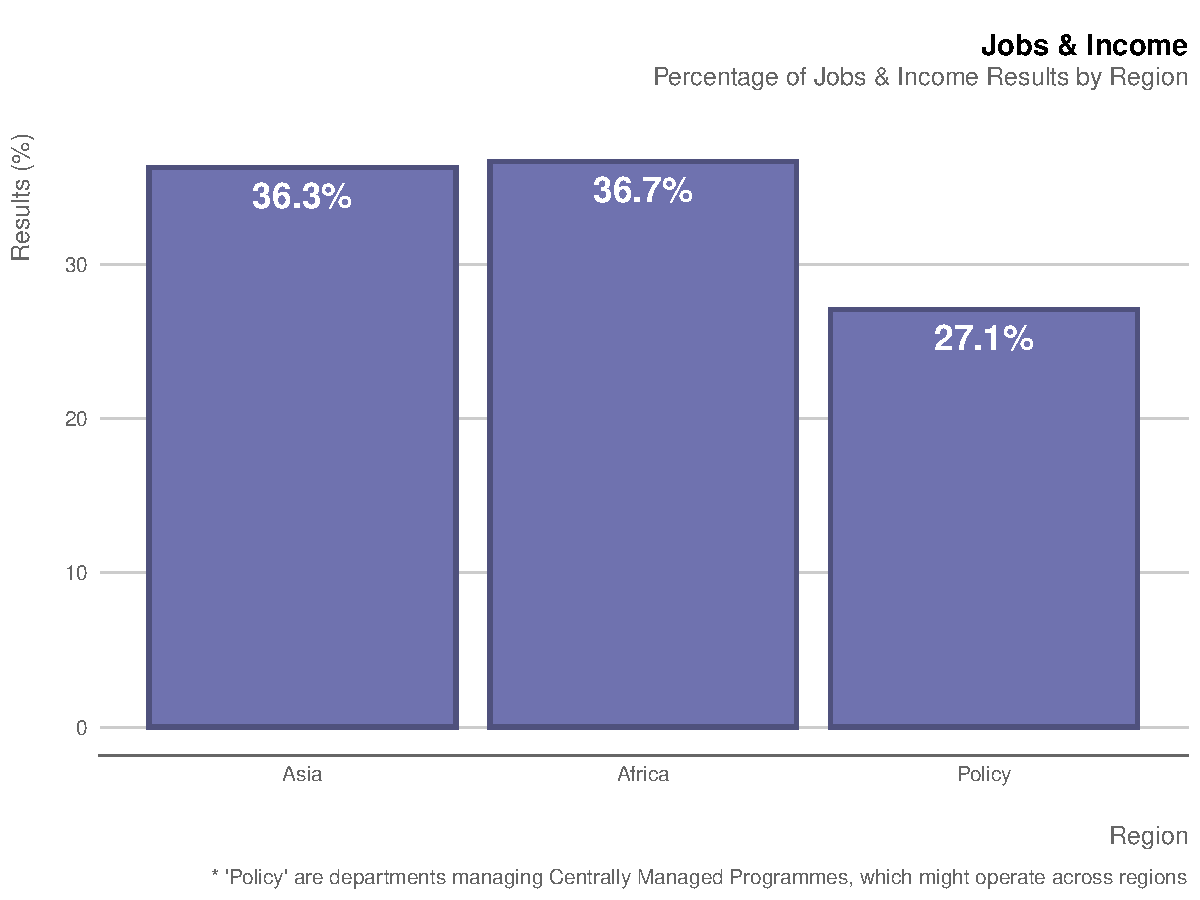
\includegraphics[width=0.8\textwidth]{../figs/jobs_region_plot} \hfill
	\caption{Percentage of Jobs and Income results by region.}
	\label{fig:jobs_region_plot}
\end{figure}



\subsection{Results by type}
Of the total 5.1 million people supported to raise their incomes or maintain/gain a better job or livelihood:

\begin{itemize}
\item 2.4 million people were supported to raise their income.
\item 1.9 million people were supported to gain or maintain a better job or livelihood. %
This includes figures for programmes which measured the number of jobs created/maintained, rather than have indicators which directly measure beneficiary numbers. %
However, a single beneficiary is assumed for every job maintained/created. %
\item The remaining 0.7 million people were beneficiaries for programmes where the indicator measured the total of all or some of the following:
	\begin{itemize}
		\item maintained income
		\item increased income
		\item maintained employment
		\item gained employment
		\item jobs created
		\item jobs supported
	\end{itemize}
\end{itemize}

Changes in the total number of people supported from previous years is affected by the composition of programmes reporting, as well as by new results from previously reporting programmes. %
Each year, new programmes may start reporting results eligible for inclusion in this indicator.  %

One significant change affecting results this year, is that we have included CDC results for the first time. %
CDC accounted for 0.85 million people supported\footnote{CDC numbers are in full-time equivalents, as per the HIPSO definition, and so are underestimates of individual beneficiaries eg seasonal and part time workers} (of which 28\% were Female and 72\% Male). %
Only beneficiary figures for 2018 (not for every year) have been included for CDC in the 2015/16 to 2019/20 DFID results. %
This is to avoid double counting the same beneficiaries who may otherwise appear in figures for multiple years. %
Note that CDC also reports indirect employment beneficiaries in supply chains, induced from wages, and enabled by productivity improvements from credit and power, estimated from the Joint Impact Model, which are not included in DFID’s aggregate figures.%


\section{Context}

DFID's overarching priority in economic development is to promote growth that creates more and better\footnote{Better jobs imply higher productivity and earnings, better benefits, better working conditions, and/or improved income protection, for example.} productive jobs and livelihoods to help people lift themselves out of poverty. %
Enhanced employment opportunities and skills is also a means to address the underlying drivers of instability and can support longer term security and stability. %

Results have been collected from 30 programmes across DFID. %T
These programmes all:
\begin{adjustwidth}{0.5cm}{}
Focused on job rich activities with an objective to either increase beneficiaries’ income from economic activity or get beneficiaries into more productive and/or better quality employment, and can provide a clear rationale of why and how the programme is doing this.
\end{adjustwidth}

\begin{adjustwidth}{8cm}{}
\textbf{AND}
\end{adjustwidth}

\begin{adjustwidth}{0.5cm}{}
The relevant jobs/income related effects on beneficiaries are monitored at least twice within the lifetime of the programme (e.g. within the logframe or regular surveys) within the existing monitoring.
\end{adjustwidth}

The exact definition of jobs/incomes is not stipulated for inclusion for this indicator as this will legitimately vary across countries, sectors and over time. %
In addition, the most suitable job/income indicator for programme monitoring will need to be programme-specific to maximise its value for monitoring. %
Following good monitoring practices, we expect indicators to be aligned with programme objectives. %

\newpage

 \chapter{Malaria: Spend}

\section*{Total UK government Official Development Assistance (ODA) spent on activities that contribute to prevention or treatment of malaria.} %

\thispagestyle{empty}

\section{Results}

In 2019/20 the total estimated UK government spend on malaria was \textbf{\pounds 429 million}. %

\section{Context}

Malaria is an infectious disease transmitted by mosquitos. %
Malaria caused an estimated 405,000 deaths in 2018 and children under the age of 5 are especially vulnerable to the disease. Most malaria cases in 2018 were in Africa (93\%) followed by South-East Asia (3.4\%)\footnote{World Malaria Report, 2018.}. %

Sustainable Development Goal 3, ``Ensure healthy lives and promote well-being for all at all age'', covers a range of health issues. %
Of the 13 targets, one (target 3.3) covers malaria specifically: ``By 2030, end the epidemics of AIDS, TB, malaria and NTDs and combat hepatitis, water-borne diseases and other communicable diseases.'' %
Progress on malaria is tracked by the SDG indicator ``Malaria incidence per 1,000 population.'' %

The UK is currently the second largest global funder of the effort against malaria\footnote{World Malaria Report, 2018.}. %
The UK contributes to the global effort on malaria through bilateral programming and funding to multilateral institutions including the Global Fund to Fight AIDS, Tuberculosis and Malaria and the World Health Organisation (WHO). %
The UK also funds research on the development of new drugs and diagnostics. %

In 2016, the then Chancellor of the Exchequer committed the UK to spend \pounds 500 million per year for five years (to 2020/21) on combating malaria. %
The then Prime Minister re-affirmed the \pounds 500 million commitment at the 2018 Commonwealth Summit. %
On 1\textsuperscript{st} July 2019, the UK government announced an up to \pounds 1.4 billion pledge to the Sixth Replenishment of the Global Fund to Fight AIDS, Tuberculosis and Malaria. %
This includes up to \pounds 200 million to double the value of private sector contributions to the Global Fund, providing \pounds 2 for every \pounds 1 contributed by the private sector. %

In 2016/17 the UK spend on malaria was \pounds 499 million, in 2017/18 the UK spend on malaria was \pounds 481 million, and in 2018/19 the UK spend on malaria was \pounds 452 million. %
These figures include all UK government funding on direct malaria programmes, multilateral contributions, research on the development of new drugs and diagnostics, and estimated contributions from wider programmes such as strengthening health systems in malaria affected countries. %


\newpage

 \chapter{Neglected Tropical Diseases: Spend}

\section*{Total UK government Official Development Assistance (ODA) spent directly on Neglected Tropical Diseases (NTD) implementation programmes or through contributions to organisations with NTD implementation activities.} %

\thispagestyle{empty}

\section{Results}

In 2019/20 the total estimated UK government spend on implementation programmes to tackle Neglected Tropical Diseases was \textbf{\pounds 52 million}. %

In 2019/20 the total estimated UK government spending on Neglected Tropical Diseases research programmes was \textbf{\pounds 31 million}. % 


\section{Context}

Neglected Tropical Diseases (NTDs) are a group of infectious diseases that affect the world's poorest and most marginalised people. %
NTDs can cause severe pain, long-term disability, chronic illness, irreversible blindness, disfiguration and death. %
Globally over one billion people are affected by these diseases and they cost developing country economies billions of dollars every year\footnote{WHO, Global Burden of Disease (GBD), 2016}. %
Some NTDs can inhibit children from learning and developing to their full potential. %
NTDs also prevent adults from working to support their families economically. %
Reaching people with preventive or curative interventions for NTDs can avoid long-term health complications or the development of disabilities. %
Large scale intervention can also reduce overall transmission of NTDs, which over time will enable their effective control or elimination\footnote{Control is the reduction of disease incidence, prevalence, morbidity, and/or mortality to a locally acceptable level. Elimination as a public health problem is defined by achievement of measurable targets set by WHO in relation to a specific disease. When reached, continued actions are required to maintain the target.}.

Sustainable Development Goal 3, ``Ensure healthy lives and promote wellbeing for all at all ages'', covers a range of health issues. %
Of the 13 targets, one (target 3.3) covers NTDs specifically: ``By 2030, end the epidemics of AIDS, TB, malaria and NTDs and combat hepatitis, water-borne diseases and other communicable diseases.'' %
Progress on NTDs is tracked by the SDG indicator ``Number of people requiring interventions against neglected tropical diseases.'' % 

In April 2017 the UK government committed to invest a total of \pounds 360 million (2017/18-2021/22) in implementation programmes to protect over 200 million people from NTDs. %
Aims of the investment include: 
\begin{itemize}
\item Wiping out (eradicating\footnote{Eradication is the permanent reduction to zero of the worldwide incidence of infection. Intervention actions are no longer needed.}) Guinea worm, which is transmitted through dirty water;
\item Preventing tens of thousands of cases of disability caused by lymphatic filariasis, a mosquito-transmitted disease which can cause severe swelling of the lower limbs; and
\item Preventing up to 400,000 cases of blindness caused by trachoma, the leading cause of infectious blindness in the world.
\end{itemize}

In addition, the UK invests in research and development for new technologies to fight NTDs. %
These research programmes are supporting the development of drugs and diagnostics for NTDs and provide evidence to improve the delivery of NTD programmes. %

This results update reports on both UK government spend on implementation programmes to tackle NTDs, to provide reporting on the commitment outlined above, and reporting of additional UK government spend on NTDs research. %

In 2018/19 the total UK government spend on implementation programmes tackling neglected tropical diseases was \pounds 44 million and in 2017/18 spend on implementation programmes was \pounds 49 million. %
In 2018/19 the total UK government spend on neglected tropical diseases research was \pounds 28 million and in 2017/18 the spend on research was \pounds 24 million. %

From 2019/20, the main vehicle for delivering the NTD spend commitment has been the \pounds 220 million Accelerating Sustainable Control and Elimination of NTDs programme (ASCEND). %
ASCEND represents a significant scale up in investment and activity and operates in twenty-five high burden countries, supporting the control and elimination of at least five NTDs. %

\newpage

 \chapter{Neglected Tropical Diseases}

\section*{Number of people receiving treatment or care for one or more neglected tropical diseases.}

\bigskip
\bigskip

% make sure numbers and header don't appear
\thispagestyle{empty}


\section{Results}

From 2017-2019 DFID reached \textbf{166.1 million} people through our Neglected Tropical Diseases (NTD) programmes.  %



\begin{table}[htbp]
	\centering
	\caption{Number of Reached by Intervention Type}\label{tab:ntd_result}
	\begin{tabular}{lr}
		\toprule
		\multicolumn{1}{c}{\textbf{Intervention Type}} & \multicolumn{1}{c}{\textbf{Number of People Reached}}\footnotemark \\ \hline

		\rule{0pt}{10pt}Preventative chemotherapy\footnotemark & 159,700,000 \\

		Other preventative measures\footnotemark & 7,500,000 \\

		Morbidity management\footnotemark & 100,000 \\

		Curative treatment\footnotemark & 10,000 \\		\bottomrule

	\end{tabular}
\end{table}

\footnotetext[32]{The total figure has been adjusted to avoid double counting individuals who may have received more than one intervention type therefore the sum of the intervention types is greater than the total of the components.}
\footnotetext[33]{Preventive chemotherapy is the treatment of entire populations at risk of infection (regardless of whether or not they are infected) to treat infection and prevent ongoing transmission.\label{ntd_note33}}
\footnotetext[34]{Other preventive measures can be used to prevent the spread of NTDs, for example water filters are used to prevent infection by Guinea Worm due to drinking contaminated water.\label{ntd_note34}}
\footnotetext[35]{Morbidity management is the provision of surgery and self-care training to address the disabling consequences of infection with lymphatic filariasis, or surgery to prevent blindness due to trachoma.\label{ntd_note35}}
\footnotetext[36]{Curative treatment is where individuals receive a diagnosis and, if infected, treatment to cure the disease.\label{ntd_note36}}

In 2017-2019 out of the total people reached by DFID's NTD interventions, 95.4\% received preventative chemotherapy\textsuperscript{33}, 0.06\% morbidity management\textsuperscript{35}, 0.01\%\textsuperscript{36} curative treatment, and 4.5\% other types of preventative measure\textsuperscript{34}. %


%\footref{\ref{ntd_note44}

\section{Context}

Neglected Tropical Diseases (NTDs) are a group of infectious diseases that affect the world's poorest and most marginalised people. %
NTDs can cause severe pain, long-term disability, chronic illness, irreversible blindness, disfiguration and death. %
Globally over one billion people are affected by these diseases and they cost developing country economies billions of dollars every year\footnote{WHO, Global Burden of Disease (GBD), 2016.}. %
Some NTDs can inhibit children from learning and developing to their full potential.  NTDs also prevent adults from working to support their families economically. %
Reaching people with preventive or curative interventions for NTDs can avoid long-term health complications or the development of disabilities. %
Large scale intervention can also reduce overall transmission of NTDs, which over time will enable their effective control or elimination\footnote{Control is the reduction of disease incidence, prevalence, morbidity, and/or mortality to a locally acceptable level. Elimination as a public health problem is defined by achievement of measurable targets set by WHO in relation to a specific disease. When reached, continued actions are required to maintain the target.}. \\%

Sustainable Development Goal 3, "Ensure healthy lives and promote well-being for all at all ages", covers a range of health issues. %
Of the 13 targets, one (target 3.3) covers NTDs specifically: "By 2030, end the epidemics of AIDS, TB, malaria and NTDs and combat hepatitis, water-borne diseases and other communicable diseases". %
Progress on NTDs is tracked by the SDG indicator "Number of people requiring interventions against neglected tropical diseases". \\%


In April 2017 the UK government committed to invest a total of \pounds 360 million (2017/18-2021/22) in implementation programmes to protect over 200m people from NTDs. %
Aims of the investment include:
\begin{itemize}
\item Wiping out (eradicating\footnote{Eradication is the permanent reduction to zero of the worldwide incidence of infection. Intervention actions are no longer needed.}) Guinea worm, which is transmitted through dirty water
\item Preventing tens of thousands of cases of disability caused by lymphatic filariasis, a mosquito-transmitted disease which can cause severe swelling of the lower limbs
\item Preventing up to 400,000 cases of blindness caused by trachoma, the leading cause of infectious blindness in the world
\end{itemize}

DFID's NTD programmes focus on lymphatic filariasis, trachoma, schistosomiasis, visceral leishmaniasis, onchocerciasis and guinea worm. %
The primary interventions used for these NTDs fall under the following categories :
\begin{itemize}
\item Preventive chemotherapy: Treatment of entire populations at risk with drugs to treat infection and prevent ongoing transmission.
\item Morbidity management: Surgery and self-care training to address swelling of limbs and genitals (for lymphatic filariasis), or surgery to prevent blindness (trachoma).
\item Curative treatments: Diagnosis and treatment of those found to be infected.
\item Other preventive measures: Other measures used to prevent transmission of infection, for example the use of cloth filters for water (Guinea Worm).
\end{itemize}

These interventions are also supported by a range of other activities, such as surveys to assess the geographical distribution of disease, disease surveillance, behaviour change communication, monitoring and evaluation, improved access to safe water, sanitation and hygiene, and vector-control. %
Table \ref{tab:ntd_impact} provides a summary of the health impacts of each of DFID's six focal NTDs, and the primary interventions applied. %


\begin{table}[htbp]
	\centering
	\caption{Health Impacts of DFID's Focal NTDs and Primary Intervention Applied.}\label{tab:ntd_impact}
	\begin{tabular}{p{0.15\linewidth}p{0.5\linewidth}p{0.25\linewidth}}
		\toprule
		\multicolumn{1}{c}{\textbf{Disease}} & \multicolumn{1}{c}{\textbf{Health Impact}} & \multicolumn{1}{c}{\textbf{Intervention}} \\ \hline
		\rule{0pt}{10pt}Lymphatic filariasis (elephantiasis) &	Abnormal enlargement of feet, legs and genitals, resulting in pain, disability and social stigma.	& Preventive chemotherapy, Morbidity management \\
		Trachoma &Eye pain and discomfort, scarring of the eyelid and cornea, causing eventual irreversible blindness. & Preventive chemotherapy, Morbidity management \\
		Schistosomiasis (bilharzia)	& Can cause liver damage, kidney failure or bladder cancer. &	Preventive chemotherapy \\
		Visceral leishmaniasis & Fever, weight loss, anaemia, and swelling of internal organs. Untreated cases usually result in death. &	Curative treatment \\
		Onchocerciasis (river blindness) & Severe itching, disfiguring skin conditions and irreversible blindness. &	Preventive chemotherapy \\
		Guinea worm & Severe pain over several weeks while worm exits leg or foot.   & Other preventive measures, Curative treatment \\
		\bottomrule
	\end{tabular}
\end{table}



\newpage

 \chapter{Nutrition}

\section*{Number of children under five, women (of childbearing age) and adolescent girls reached by DFID through nutrition-related interventions.}

\thispagestyle{empty}



\section{Results}

From 2015-2020 DFID reached \textbf{
55.1 million
} children under 5, women of childbearing age and adolescent girls through our nutrition-relevant programmes. %

\begin{figure}[htbp]
	\centering
\begin{knitrout}
\definecolor{shadecolor}{rgb}{0.969, 0.969, 0.969}\color{fgcolor}
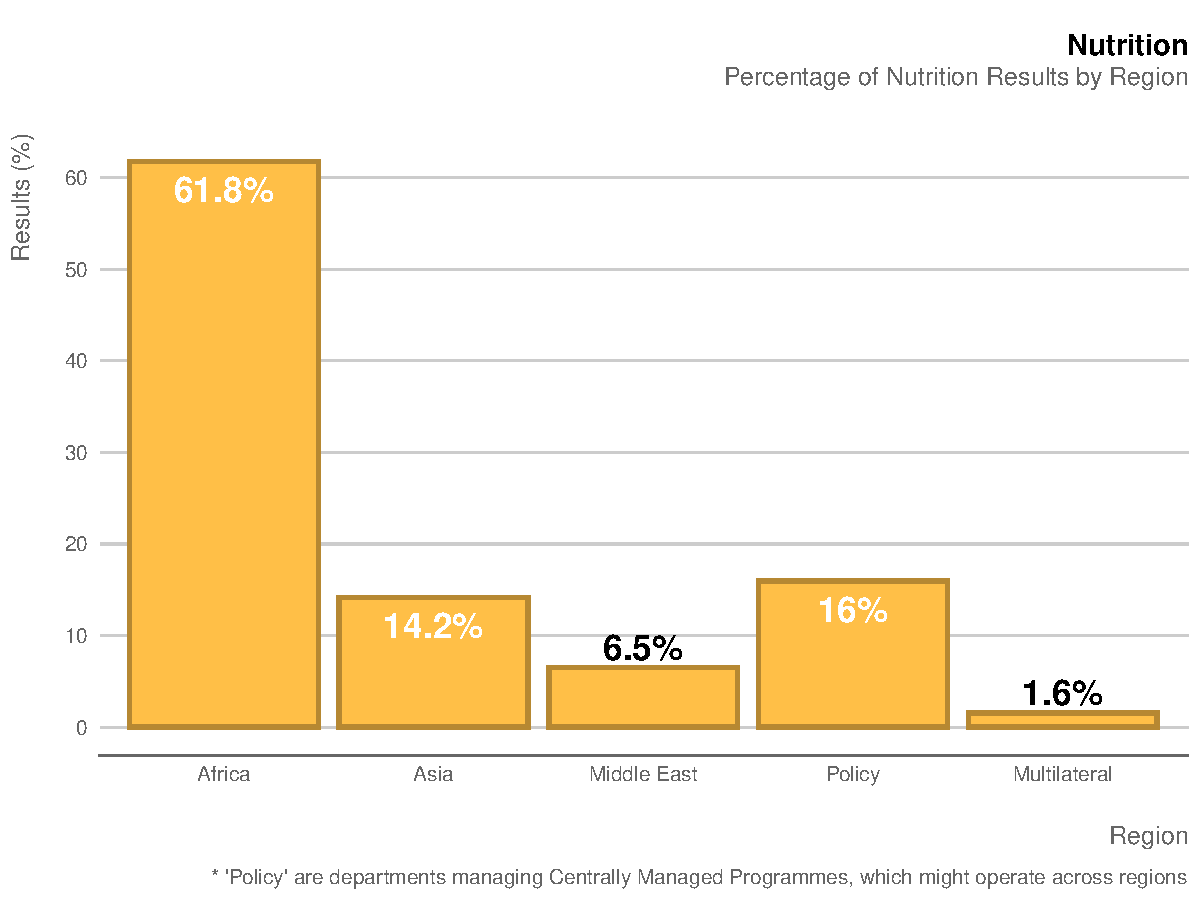
\includegraphics[width=0.8\textwidth]{figs/nutrition_region_plot-1} 

\end{knitrout}
	%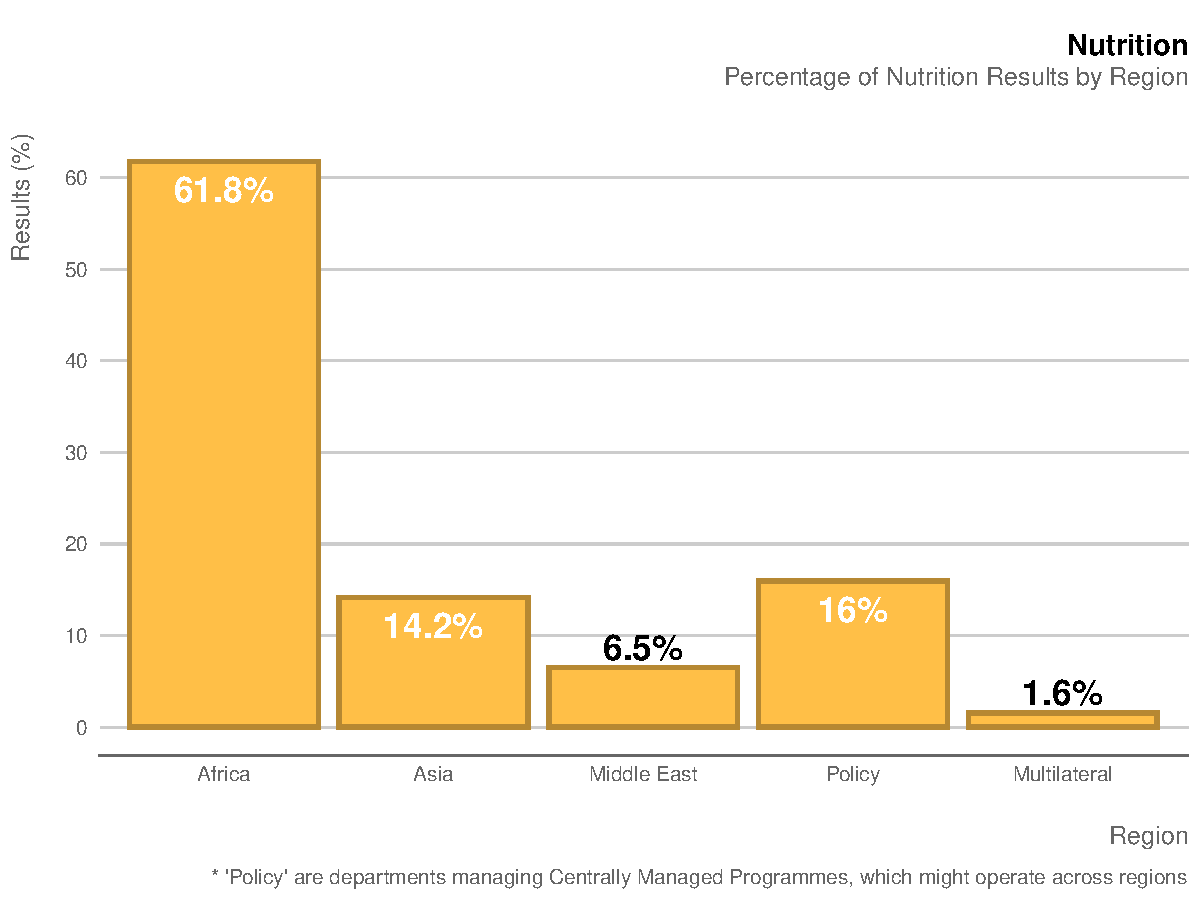
\includegraphics[width=0.8\textwidth]{../figs/nutrition_region_plot} \hfill
	\caption{Percentage of Nutrition results by region.}\label{fig:nutrition_region_plot}
\end{figure}


From 2015 to 2020, Africa was the largest beneficiary of DFID's nutrition-related programmes, with 37.5 million beneficiaries reached (see Figure \ref{fig:nutrition_region_plot} for regional percentage breakdown). %
DFID reached 8.6 million beneficiaries in Asia: the majority of whom were in Bangladesh (6.1 million). %
DFID reached 3.9 million beneficiaries in the Middle East: the majority of whom were in Yemen (3.5 million). %
A further 10.6 million beneficiaries of DFID's nutrition results were delivered via non-country or -region specific programmes, and multilateral organisations. %

Most of the children under 5, women of childbearing age and adolescent girls (48.4 million
beneficiaries) reached by DFID's nutrition-related programmes live in fragile states (using the OECD States of Fragility definition), including 15.2 million beneficiaries living in Extremely Fragile States (Figure \ref{fig:nutrition_fragility_plot}). %

\begin{figure}[htbp]
	\centering
\begin{knitrout}
\definecolor{shadecolor}{rgb}{0.969, 0.969, 0.969}\color{fgcolor}
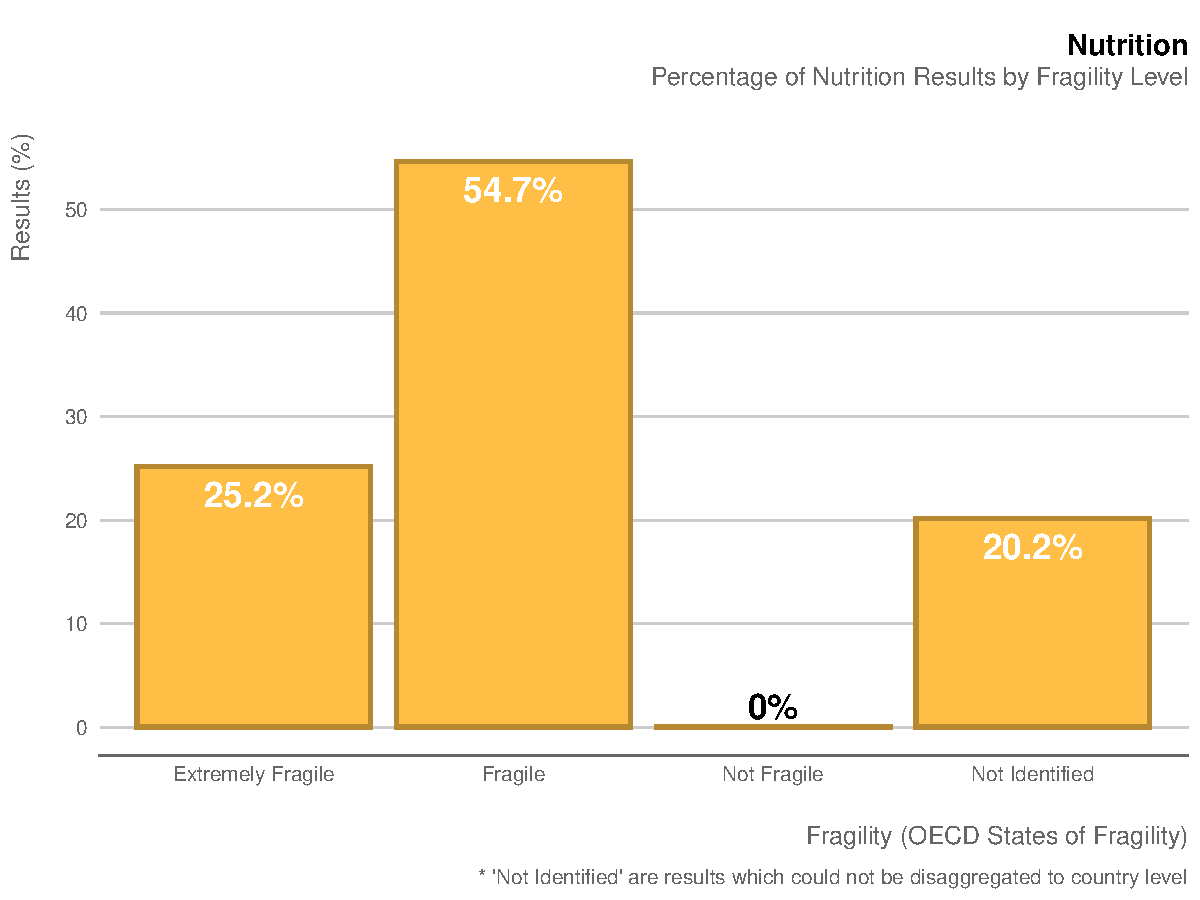
\includegraphics[width=0.8\textwidth]{figs/nutrition_fragility_plot-1} 

\end{knitrout}
	%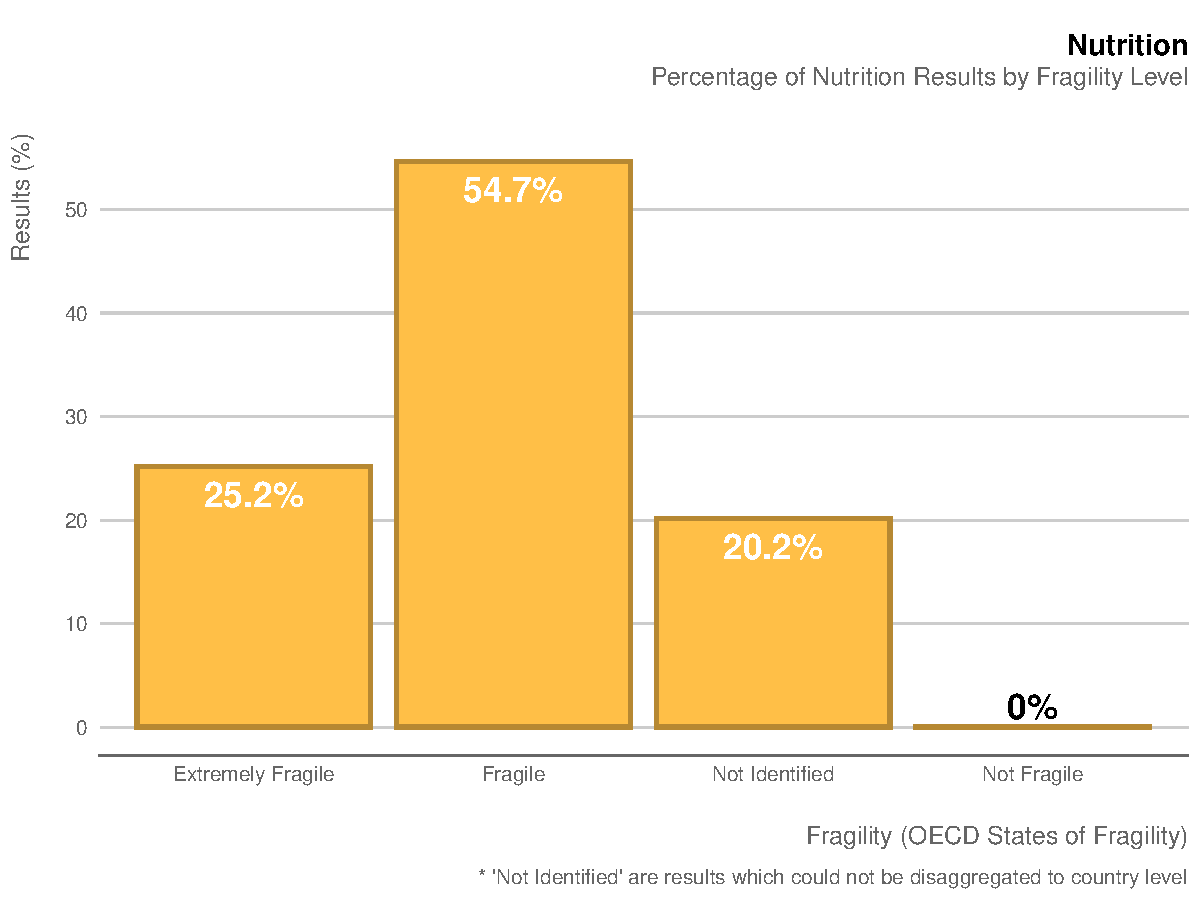
\includegraphics[width=0.8\textwidth]{../figs/nutrition_fragility_plot} \hfill
	\caption{Percentage of Nutrition results by fragility level.}\label{fig:nutrition_fragility_plot}
\end{figure}


High, medium and low intensity results are defined according to:
\begin{itemize}
	\item Comprehensiveness of the package reaching the target population
	\item Whether this package is directly or indirectly targeted to this target population
\end{itemize}

In all cases, `target population' refers to women of childbearing age (15 to 49 years), children under 5 years and adolescent girls (10 to 19 years). %
Please refer to the methodology summary, and the published methodology note for more details. %

\begin{figure}[htbp]
	\centering
\begin{knitrout}
\definecolor{shadecolor}{rgb}{0.969, 0.969, 0.969}\color{fgcolor}
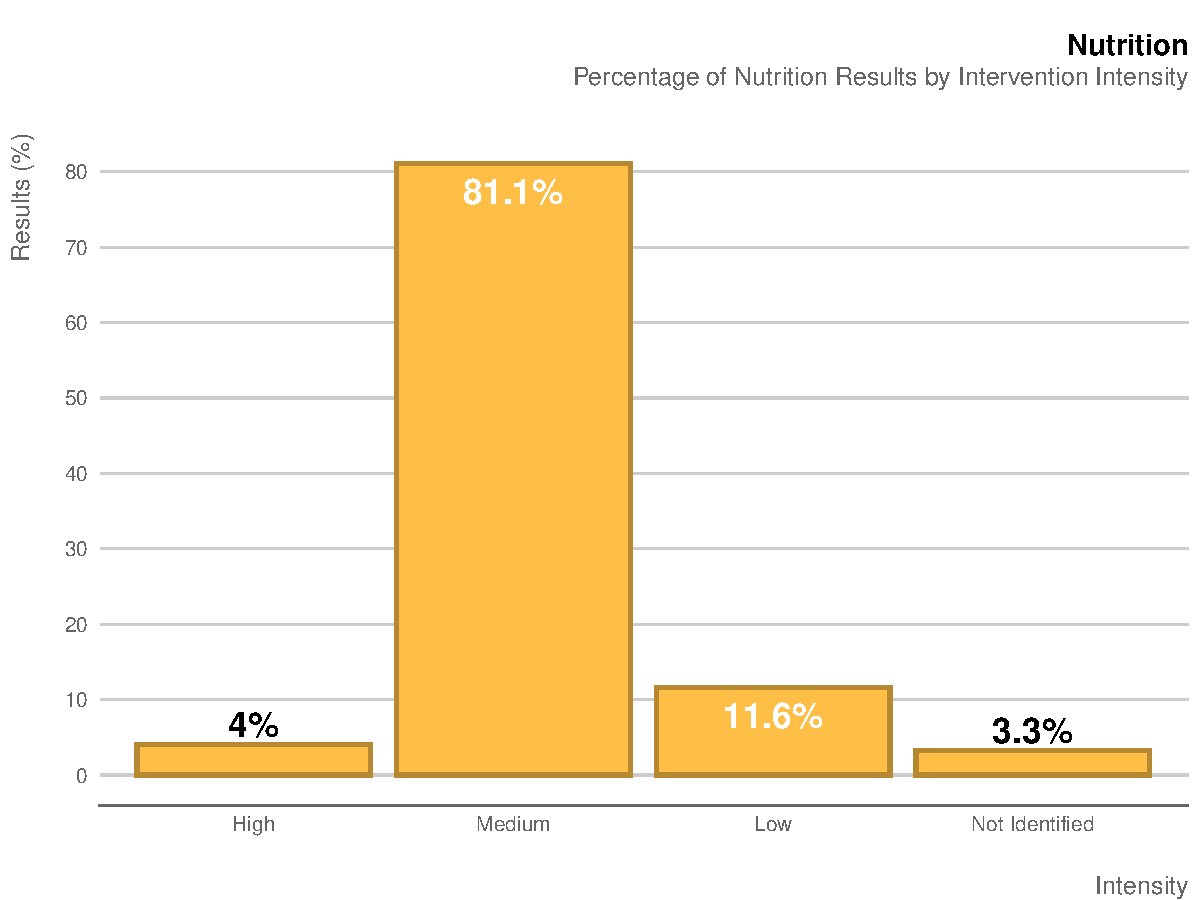
\includegraphics[width=0.8\textwidth]{figs/nutrition_intensity_plot-1} 

\end{knitrout}
	%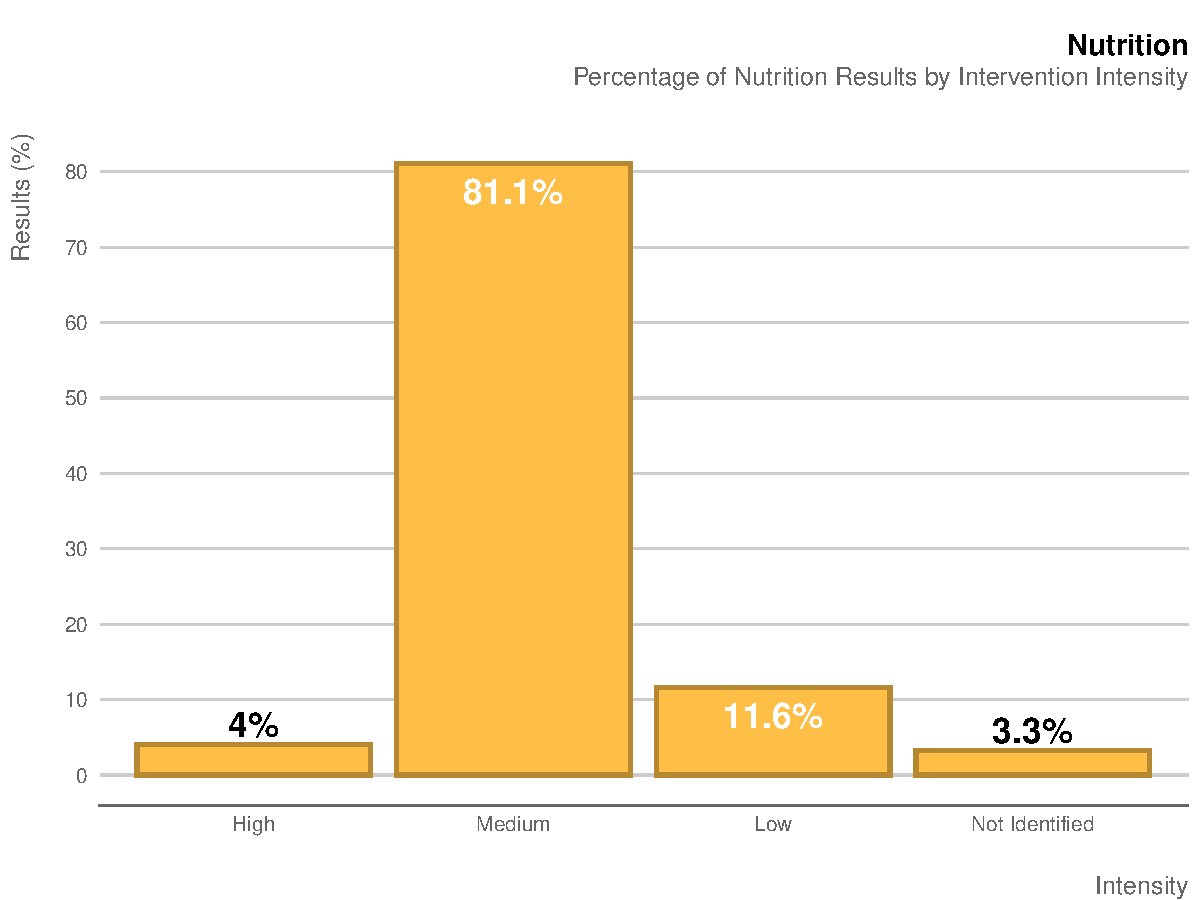
\includegraphics[width=0.8\textwidth]{../figs/nutrition_intensity_plot} \hfill
	\caption{Percentage of Nutrition results by intervention intensity.}\label{fig:nutrition_intensity_plot}
\end{figure}

The approach to calculating nutrition results has been updated this year as part of or comittment to continuously improve the quality of our results estimates, incorporating the latest available data and reducing the risk of double counting. %
These improvements show a shift in the pattern of the intensity of the interventions we delivered, compared to the last updated data published on 28th January 2020. %
There has been a decrease in the proportion of high and low internsity interventions and an increase in the proportion of medium intensity interventions we delivered. %
Most of the beneficiaries of DFID nutrition-related programmes have received medium intensity interventions (49.9 million
beneficiaries; Figure \ref{fig:nutrition_intensity_plot}). %
DFID nutrition-related programmes reached 2.4 million beneficiaries with high intensity intervention and 7.1 million beneficiaries with low intensity interventions. %
Intensity information was not available for 2 million beneficiaries of DFID's nutrition results\footnote{The total number beneficiaries counted from the different intensities of intervention may exceed the overall total number of beneficiaries reached on Page 1. This is due to the application of the peak year method at the country level: the overall total achieved counts the single year with the largest number of results within a country. Since the ``peak'' reach within a country may occur in different years for each intensity level, the total achieved by intensity may sum across different years, resulting in a larger reach than the overall total.}. %

Of those reached by DFID nutrition-related programs from 2015 to 2019, 24 million were women and girls. %
DFID is continuously working with our existing partners towards improving collection of disaggregated data. %
In 2018/19 50\% of our reported nutrition results were disaggregated by gender. %


\section{Context}

Good nutrition plays a key role in child development. Children who are undernourished are more likely to get sick or die. %
Those who survive suffer impaired physical growth and brain development, which limits educational attainment and lifelong earning potential. %
Under-nutrition remains a major challenge in developing countries including those that face humanitarian crises. %

Globally, there are an estimated 144 million children under 5 who are stunted (too short for their age, which can limit brain development) and 47 million who are wasted (low weight for their height, which can increase the risk of death) due to poor nutrition\footnote{UNICEF/WHO/World Bank Group (2020). Joint Child Malnutrition Estimates 2018 edition. New York. Available at: \href{https://data.unicef.org/resources/jme/}{https://data.unicef.org/resources/jme/}}. %
The greatest burden of undernutrition falls within Africa and Asia, with almost one in three children in Africa suffering from stunting, and almost one in four children in Asia. %
Sustainable Development Goal 2 aims to end hunger, achieve food security and improved nutrition and promote sustainable agriculture, and includes a specific target to end all forms of malnutrition by 2030. %
The recent pace of change is insufficient to meet this target, and in some countries no progress or a worsening of the situation has been seen\footnote{Development Initiatives (2017). Global Nutrition Report 2017: Nourishing the SDGs. Bristol: Development Initiatives. Available at: \href{https://www.globalnutritionreport.org/files/2017/11/Report_2017.pdf}{https://www.globalnutritionreport.org/files/2017/11/Report\_2017.pdf}}. %

Interventions to improve nutrition among children, adolescent girls and women of childbearing age can result in a return on investment of \pounds 16 for every \pounds 1 spent\footnote{Hoddinott, J (2016). Global Panel on Agriculture and Food Systems for Nutrition Working Paper: The economics of reducing malnutrition in Sub-Saharan Africa. Available at: \href{http://glopan.org/sites/default/files/Global_Panel_Working_Paper.pdf}{http://glopan.org/sites/default/files/Global\_Panel\_Working\_Paper.pdf}}. %
The 2013 Lancet Commission on Maternal and Child Nutrition recommended the scale-up of a package of ten key interventions to directly address the causes of under-nutrition (the so-called nutrition-specific package), based on the available evidence of efficacy\footnote{Bhutta, Z.A. et al. (2013). Evidence-based interventions for improvement of maternal and child nutrition: what can be done and at what cost? The Lancet, Volume 382, Issue 9890, pp. 452-477}. %
It was estimated that 90\% coverage of these interventions could reduce under-five deaths by 15\%. %
However, scale-up of the nutrition-specific package alone will only address 20\% of the burden of stunting, given the influence of a range of other factors on child stunting. %
To address the remaining 80\% of the stunting burden, cross-sectoral actions (nutrition-sensitive interventions) are required to address the underlying determinants of under-nutrition\footnote{Ruel, M.T. et al. (2013). Nutrition-sensitive interventions and programmes: how can they help to accelerate progress in improving maternal and child nutrition? The Lancet, Volume 382, Issue 9891, pp. 536-551}. %

\newpage

 \chapter{Official Development Assistance (ODA)}

\section*{An overview of official UK spend on international development and the UK target to spend 0.7\% of gross national income per calendar year.}

\thispagestyle{empty}



\section{Results}

In 2019 provisional ODA spend\footnotemark represented \textbf{
0.7\%
} of UK Gross National Income (GNI). %
The total amount of ODA provided by the UK Government was provisionally \textbf{\pounds
15,174 million
} in 2019. %
This was an increase of \pounds
622
million
(4.1\%) on spend in 2018 (\pounds
14,552 million). %

\footnotetext{In 2018, a grant equivalent basis for ODA is measurement was introduced.}

Figure \ref{fig:oda_gni_plot} shows the trend in UK ODA since 1970. %
Overall there has been a steady increase in the level of UK ODA since 1970, with a peak in 2005 and 2006 which was driven by high levels of debt relief, and a steep increase in 2013 when the UK Government first met the 0.7\% ODA:GNI target. %

The jump in the level of ODA in 2016 reflects the switch to the European System of Accounts (ESA) 2010 methodology for measuring GNI and the consequent need to increase UK ODA to meet the 0.7\% ODA target. %


\begin{figure}[htbp]
  \centering
\begin{knitrout}
\definecolor{shadecolor}{rgb}{0.969, 0.969, 0.969}\color{fgcolor}
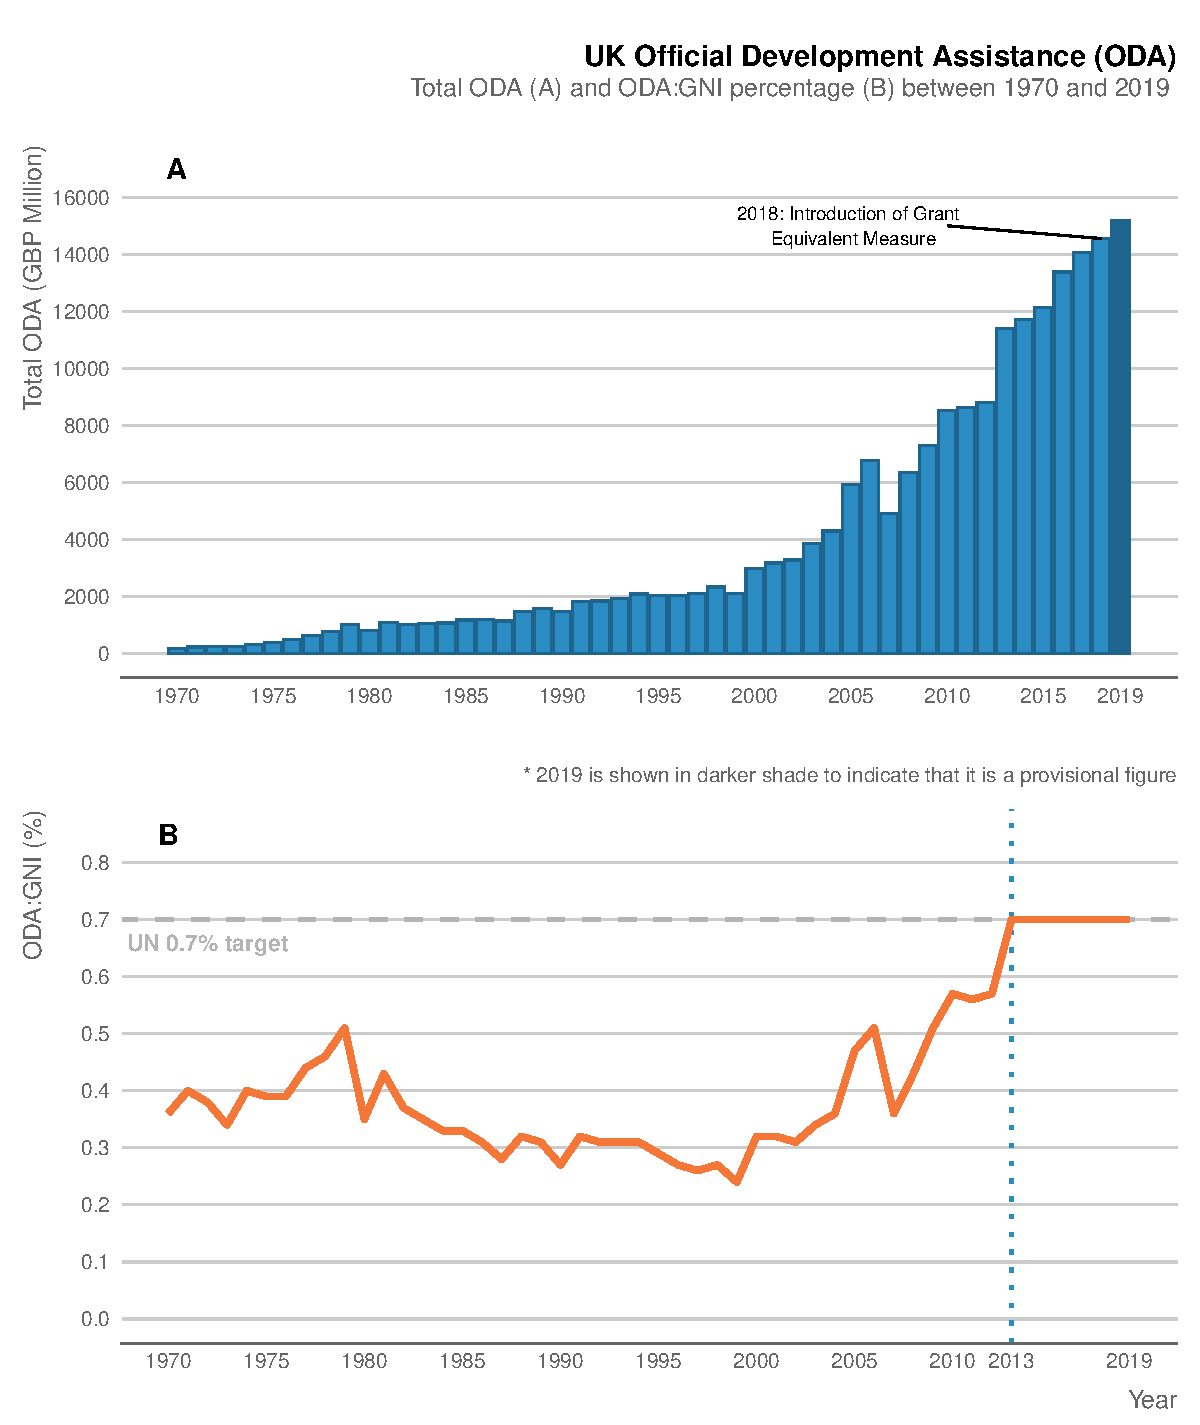
\includegraphics[width=0.9\textwidth]{figs/oda_gni_plot-1} 

\end{knitrout}
  %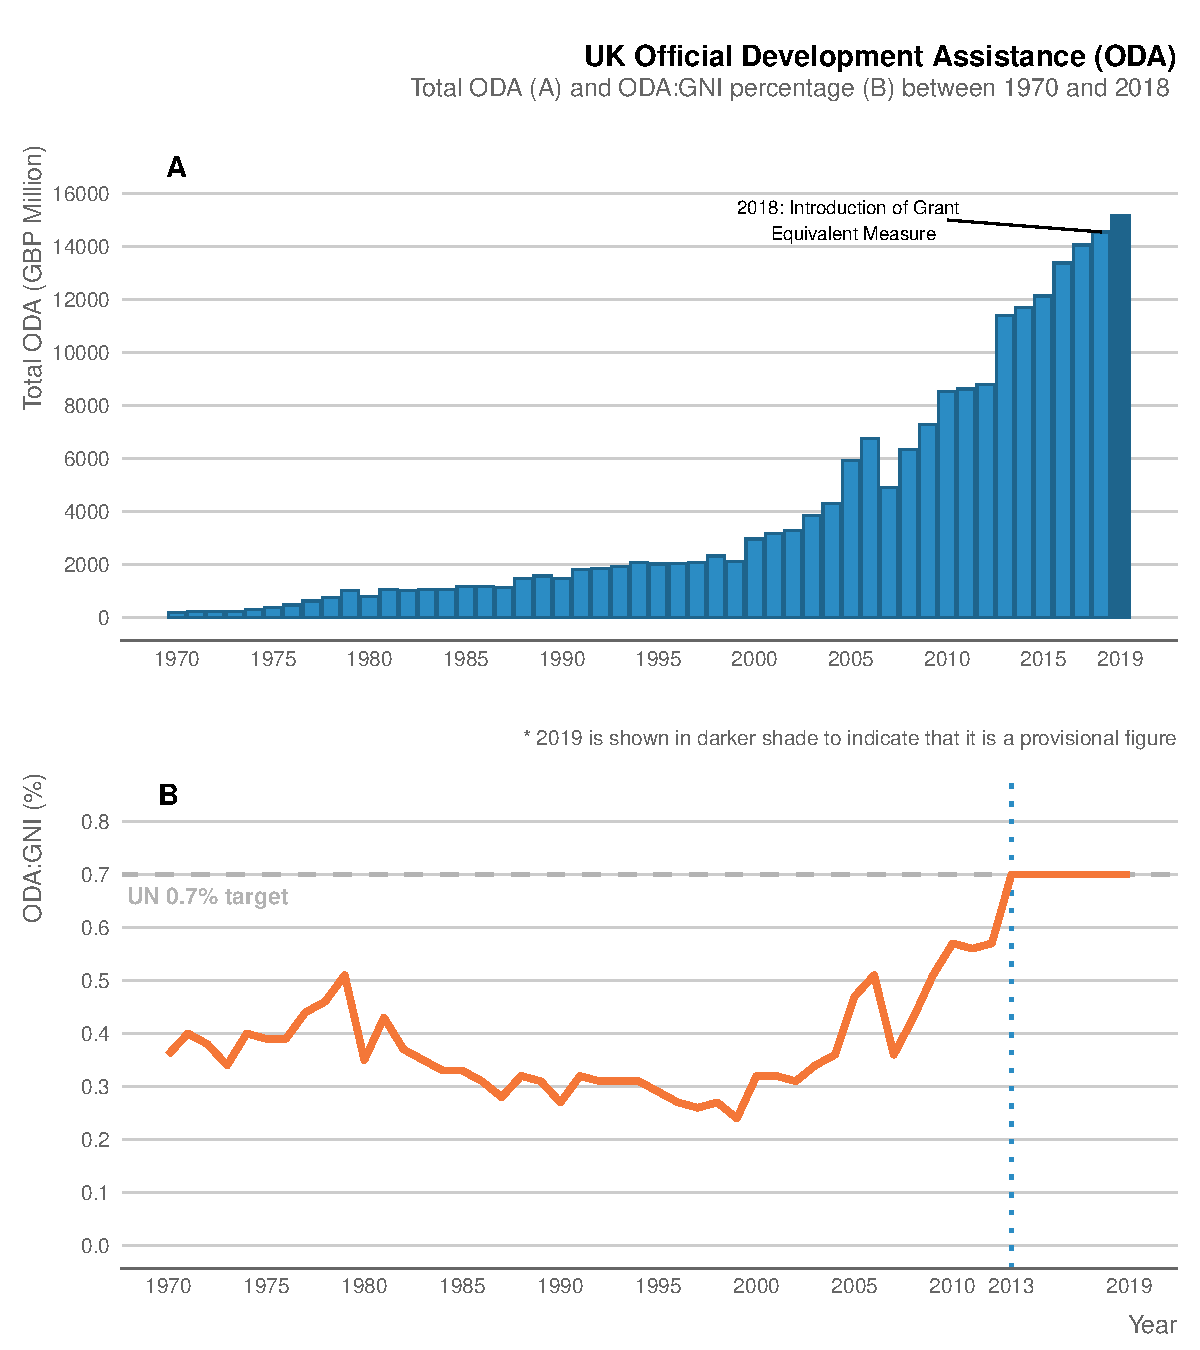
\includegraphics[width=1\textwidth]{../figs/oda_gni_plot} \hfill
  \caption{UK ODA level and ODA as a percentage of GNI between 1970 and 2019.}
  \label{fig:oda_gni_plot}
\end{figure}

For more information on UK aid spending please follow link to DFID's national statistics publication \href{https://www.gov.uk/government/statistics/statistics-on-international-development-provisional-uk-aid-spend-2019}{Statistics on International Development: UK Aid Spend 2019}. %

\section{Context}

The United Nations General Assembly agreed on an international target of 0.7\% for the ODA:GNI ratio in 1970. %
The UK government first made a commitment to increase total UK ODA to 0.7\% of GNI by 2013, and in 2015 the commitment was enshrined in UK law. %

\newpage


 \chapter{Portfolio Quality Index}

\section*{}


\thispagestyle{empty}


\section{Results}
The Portfolio Quality Index (PQI) increased from 103.8 in April 2019 to \textbf{104.5} in March 2020. %
During 2019-20, the lowest was 103.0 in October 2019 and the highest was 104.8 in December 2019. %


\section{Context}
DFID uses an index of portfolio quality to measure the extent to which projects are on track to deliver their expected outputs. %
The PQI provides a measure of how well the aggregate portfolio of projects (weighted by value of project) is performing, with a range from 50 (outputs substantially did not meet expectation) to 150 (outputs substantially exceeded expectation). %


\newpage

 \chapter{Private Sector Investment}

\section*{}


\thispagestyle{empty}


\section{Results}

Private Investment Development Group (PIDG) estimate they mobilised an additional \textbf{\pounds 1.6 billion} in private investment in the year 2019 (PIDG report results in calendar years). \\%
  
\noindent CDC estimate they mobilised an additional \textbf{US\$0.8 billion} in 2019. %
The PIDG and CDC figures use different methodologies and so are not comparable. %


\begin{table}[htbp]
  \centering
  \caption{PIDG and CDC annual breakdowns of results (\pounds billion)}\label{tab:private_pidg}
  \begin{tabular}{lc}
    \toprule
    \multicolumn{2}{c}{\textbf{PIDG}} \\ \hline
    \multicolumn{1}{c}{\textbf{Year}} & \textbf{Amount} (\pounds bn) \\ \hline
    \rule{0pt}{10pt}2015 & 1.7 \\
    2016 & 1.6 \\
    2017 & 1.6 \\
    2018 & 2.0 \\ 
    2019 & 1.6 \\ \bottomrule
  \end{tabular}
    \hspace{1em}
  \begin{tabular}{lc}
    \toprule
    \multicolumn{2}{c}{\textbf{CDC}}  \\  \hline
    \multicolumn{1}{c}{\textbf{Year}} & \textbf{Amount} (\pounds bn) \\  \hline
    \rule{0pt}{10pt}2015 & 1.5 \\
    2016 & 1.1 \\
    2017 & 0.7 \\
    2018 & 0.5 \\ 
    2019 & 0.8 \\ \bottomrule
  \end{tabular}
\end{table}



\section{Context}

The additional financing needed to achieve the UN Sustainable Development Goals by 2030 is estimated at \$2.5 trillion every year, but current investment levels are less than half of that. %
As the UN made clear, much of this finance needs to come from the  private sector. The Department, investing through CDC and the various PIDG facilities, supports the growth of businesses and new infrastructure projects in Africa and South Asia that would otherwise go unfunded. %
By providing patient capital, CDC and PIDG help to `crowd in' private finance by reducing the risks borne by others who invest alongside them. %
By pioneering successful investments in sectors and geographies deemed too risky by private sector investors, they demonstrate that it is possible to invest responsibly in these markets and earn a financial return, helping to overcome the barriers that currently deter investment capital from flowing into those countries that desperately need it. %

\newpage

 \chapter{Progress Towards Polio Eradication}

\section*{Number of global wild poliovirus cases.}

\bigskip
\bigskip

% make sure numbers and header don't appear
\thispagestyle{empty}

\section{Results}
DFID supports the Global Polio Eradication Initiative (GPEI) to eradicate polio, with \textbf{175 cases} of wild poliovirus (WPV) globally in 2019. \\%

\noindent\textbf{The number of wild polio cases has been reduced from 350,000 in 1988, to 175 in 2019}\footnote{\href{http://polioeradication.org/polio-today/polio-now/this-week/}{http://polioeradication.org/polio-today/polio-now/this-week/}}. \\%

In 2019, Afghanistan reported 29 cases and Pakistan reported 146 cases. %
Nigeria has not reported a case since August 2016 and discussions are ongoing about declaring the country, and the African Continent, free from WPV. \\%

An increase of 142 cases between 2018 (in which there were 33 cases) and 2019 was the result of severe insecurity and inaccessibility in certain parts of the endemic countries, as well as the spread of misinformation about the vaccine that prevented GPEI from performing vaccination campaigns and reduced vaccine uptake. %
The GPEI is working with a wide range of actors to improve access and build trust with local communities in the affected regions. %


\section{Context}

Polio is a highly infectious viral disease which primarily spreads from person to person, usually by the faecal-oral route. %
It causes irreversible paralysis in around 1 in 200 cases, most of whom are children under five years old. %
Among those paralysed, 5\% to 10\% will die. %
There is no cure for polio, but there are safe and effective vaccines. \\%

Since its inception in 1988, the GPEI, which is a partnership of World Health Organisation (WHO), United Nations Children's Fund (UNICEF), the Bill \& Melinda Gates Foundation, the US Center for Disease Control, Gavi the Vaccine Alliance \& Rotary International, has successfully led global efforts that have reduced Wild Polio Virus (WPV) cases by more than 99\% from 350,000 cases a year in 125 countries, to 175 cases, in 2019, with only three countries not yet certified wild polio-free (Afghanistan, Nigeria, Pakistan). \\%

The UK is currently the second largest state donor to the GPEI and is also the largest donor to Gavi, the Vaccine Alliance, which funds the Inactivated Polio Vaccine (IPV). %

\newpage

 \chapter{Public Financial Management}

\section*{Number of countries supported by DFID to manage their public finances (including natural resources and extractives) more transparently.}
% make sure numbers and header don't appear
\thispagestyle{empty}



\section{Results}

In 2019/120 DFID supported \textbf{39 countries} to manage their public finances (including natural resources and extractives) more transparently. %
This compares with 40 countries in 2018/19 and 39 countries in 2017/18. %

From 2015 to 2020 DFID continuously supported 26 countries to manage their public finances (including natural resources and extractives) more transparently.
%

\begin{figure}[htbp]
  \centering
\begin{knitrout}
\definecolor{shadecolor}{rgb}{0.969, 0.969, 0.969}\color{fgcolor}
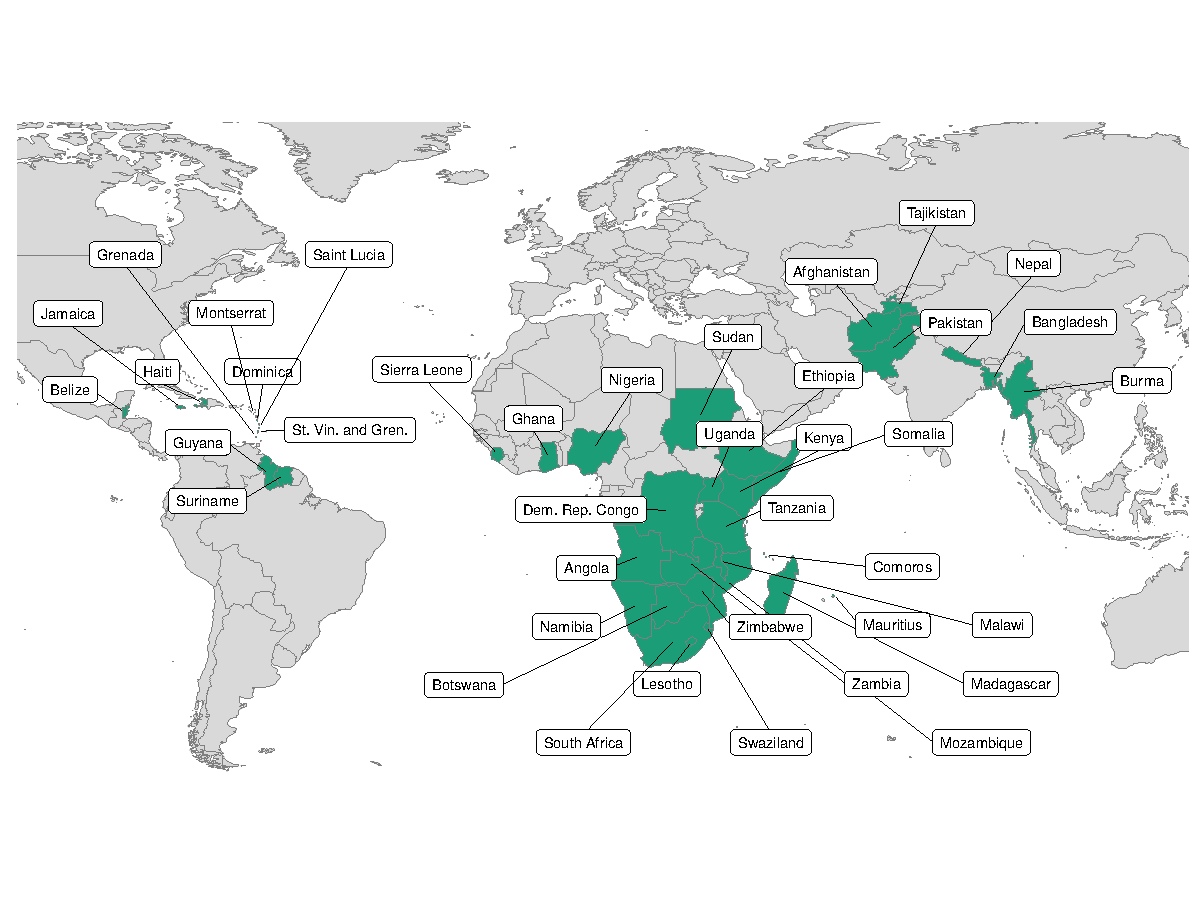
\includegraphics[width=0.9\textwidth]{figs/pfm_plot-1} 

\end{knitrout}
  %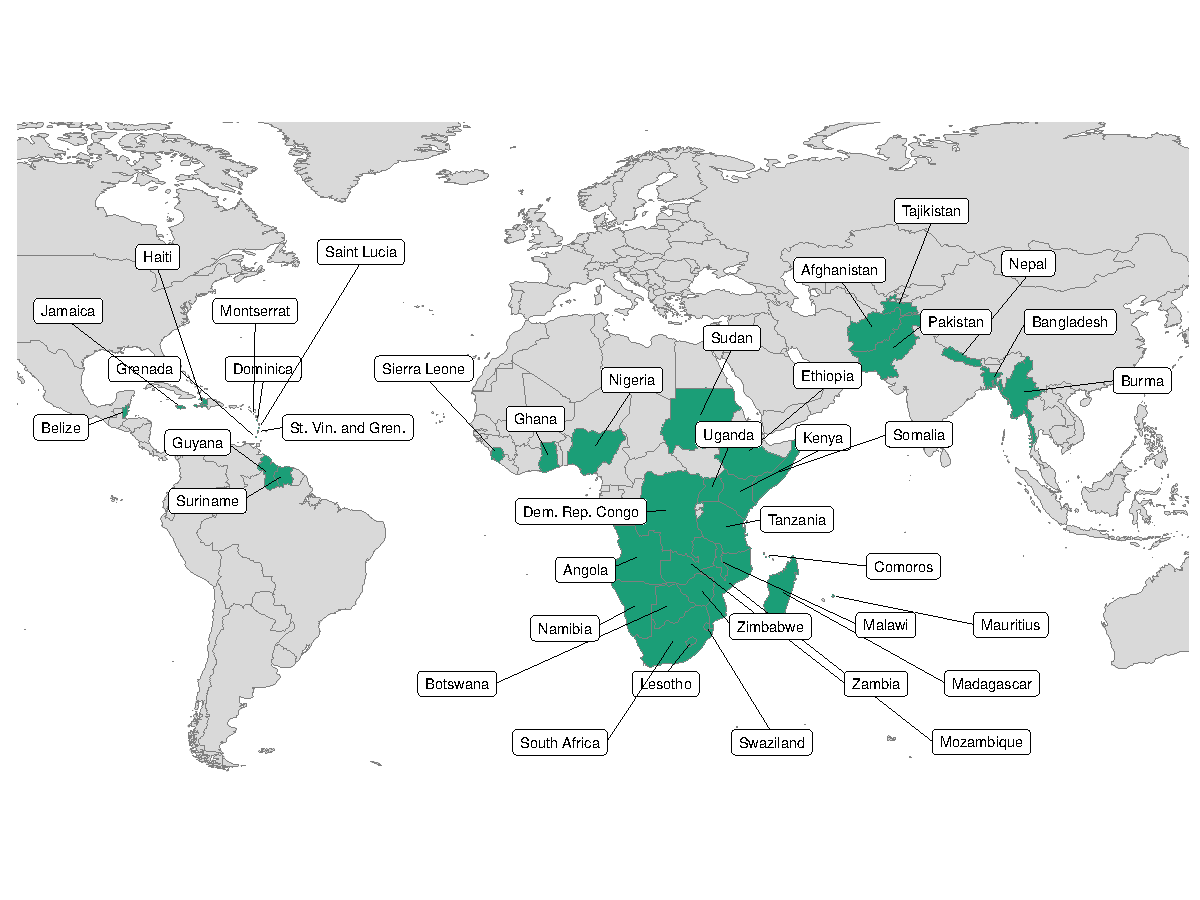
\includegraphics[width=0.95\textwidth]{../figs/pfm_plot} \hfill
  \caption{Countries supported in 2019/20 to manage their public finances more transparently.}
  \label{fig:pfm_plot}
\end{figure}


\section{Context}

Developing countries need to raise and use their own revenues to finance public services, and enable sustainable and inclusive growth and poverty reduction. %
Lack of transparency over Government budgeting makes it difficult to track spending, detect
misuse of public funds and hold decision makers to account. %

DFID support to improve fiscal transparency and accountability in developing countries is vital for a sustainable exit from aid, develops strong defence against corruption, and helps build capable and legitimate states, which are core to DFID's approach. %
This work also contributes towards delivery of the Sustainable Development Goals,
particularly Goal 16 (building `more effective and transparent institutions'). %

\newpage


 \chapter{Water, Sanitation and Hygiene}

\section*{Number of people with sustainable access to clean water and/or sanitation through DFID support.}
% make sure numbers and header don't appear
\thispagestyle{empty}

\section{Results}

Between 2015 and 2020 DFID has supported \textbf{62.6 million} people to gain access to clean water and/or better sanitation. %

\begin{figure}[htbp]
	\centering
	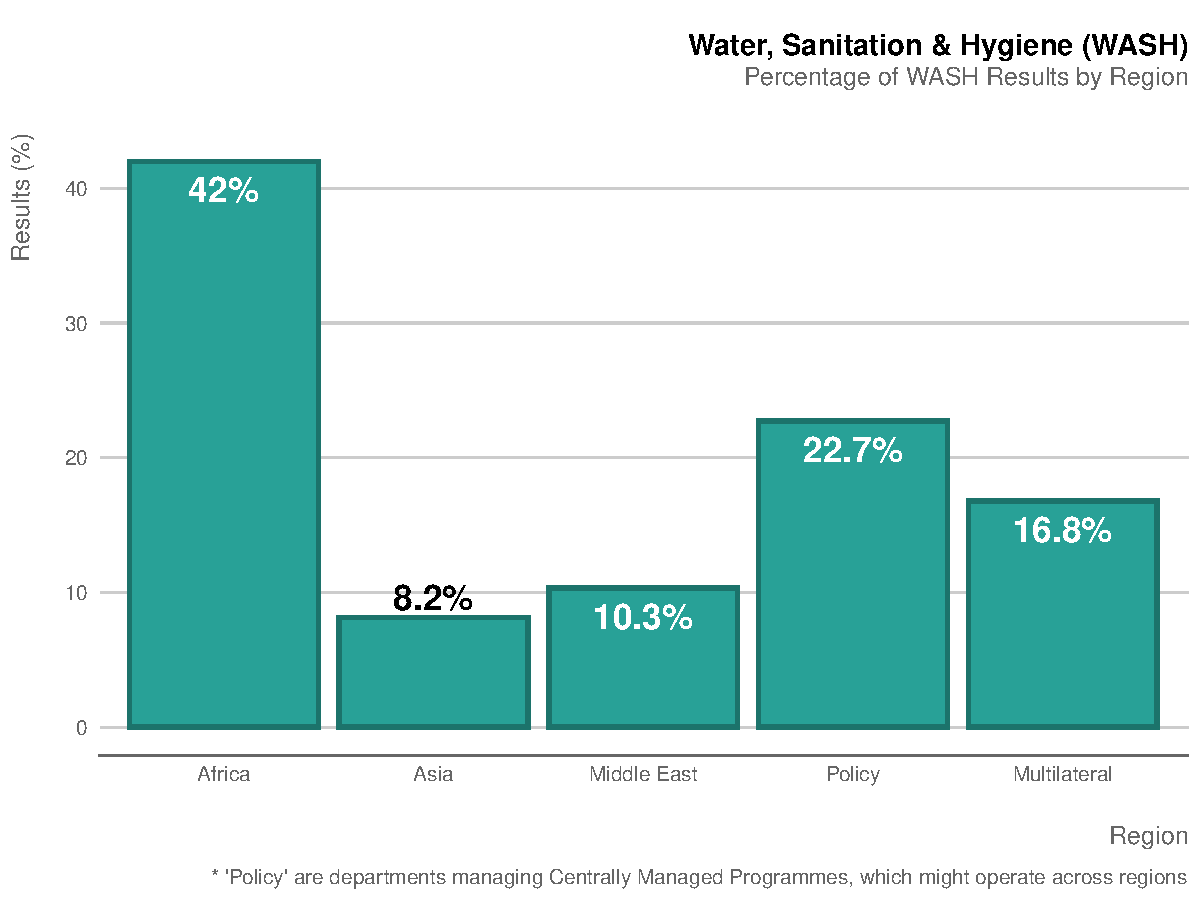
\includegraphics[width=0.8\textwidth]{../figs/wash_region_plot} \hfill
	\caption{Percentage of WASH results by region.}
	\label{fig:wash_region_plot}
\end{figure}


From 2015 to 2020, Africa was the largest beneficiary of DFID Water Supply, Sanitation and Hygiene (WASH) programmes, with 26.3 million beneficiaries reached. %
DFID also reached over 6 million beneficiaries in the Middle East --- the majority of whom were in Syria (4.9 million) --- and 5.1 million beneficiaries in Asia. %
A further 39\% (24.7 million beneficiaries) of DFID's WASH results were delivered via non-country specific programmes, non-region-specific programmes, and multilateral organisations. %

\begin{figure}[htbp]
	\centering
	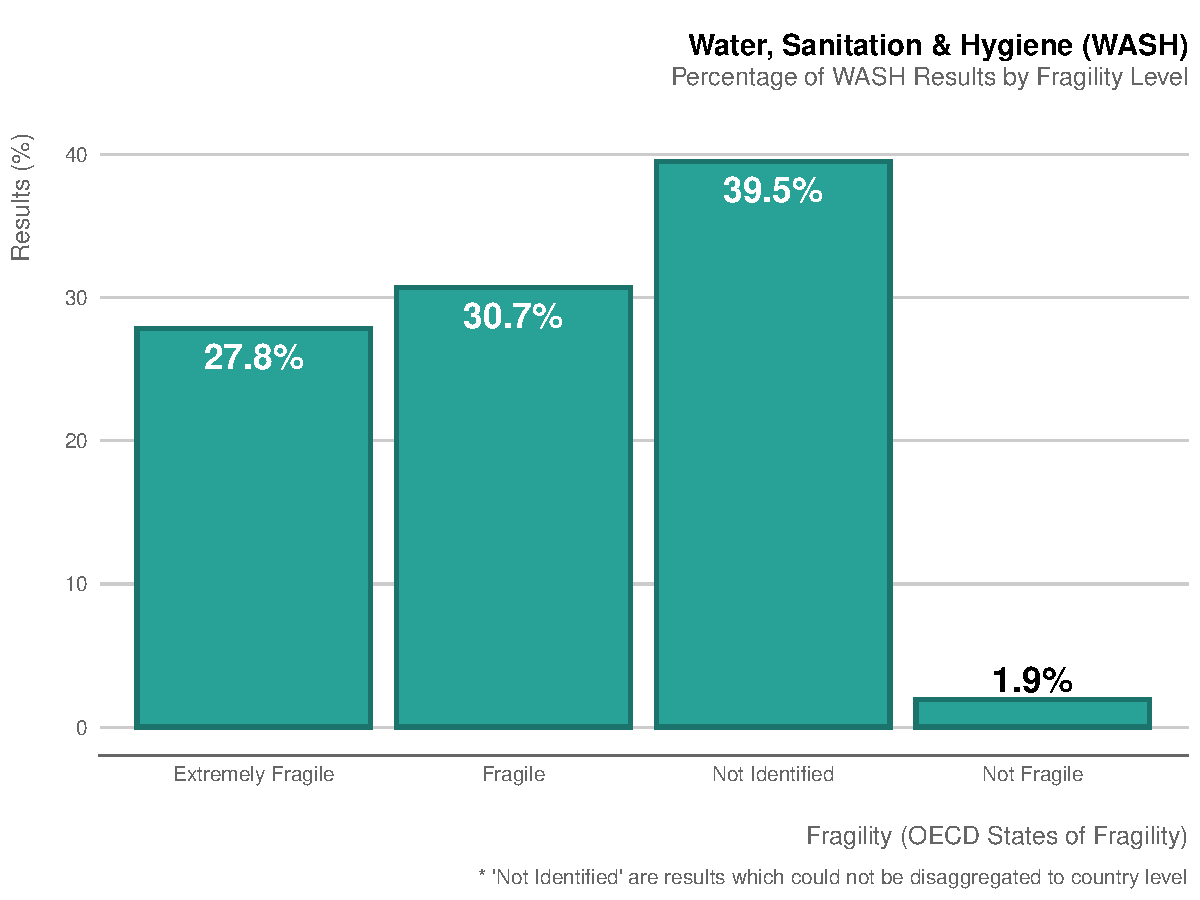
\includegraphics[width=0.8\textwidth]{../figs/wash_fragility_plot} \hfill
	\caption{Percentage of WASH results by fragility level.}
	\label{fig:wash_fragility_plot}
\end{figure}

DFID uses the OECD definition of fragile states, which is used to ensure we focus resources in the most fragile and conflict-affected countries. %
Most of the population reached by DFID WASH programs live in fragile states (37.8 million beneficiaries), including 17.4 million beneficiaries living in extremely fragile states. %

Of the results that have been disaggregated by gender from 2015 to 2020, DFID WASH programs reached 24.1 million women. %
In 2019/20 75\% of our reported WASH results were disaggregated by gender. %
This is a 4-percentage point increase in data disaggregation by gender between the results reported in 2018/19 and the results reported in 2019/20. %

\section{Context}
Successive governments have emphasised the importance of water supply and sanitation to support broader objectives for health, well-being and economic development. %
The November 2019 Conservative Party manifesto committed to build on existing efforts to end preventable deaths of mothers, new-borns and children  by 2030. %
Water supply, sanitation and hygiene are all necessary elements to secure the health outcomes that would meet this ambition. %
For example, safe water and sanitation is the most effective way of preventing 1,000 young children dying every day from diarrhoea. %

WASH is also critical in managing epidemic diarrhoeal diseases such as cholera as well as some of the most prevalent neglected tropical diseases, including trachoma, schistosomiasis and soil transmitted helminths. %

The provision of safe water, sanitation and hygiene is essential in protecting human health during the COVID-19 outbreak. %
We know the disease is highly infectious and can spread rapidly. %
Frequent and proper hand hygiene is therefore one the most important prevention measures for COVID-19 but requires sufficient availability of water. %

The non-health benefits of WASH are equally significant, especially for improving the lives of women and girls whose education and future prosperity can suffer from, for example, bearing the burden of collecting water. %

Based on 2016 data – the most recent available, 31\% of schools lack basic water supplies --- needed not only for drinking but also to keep toilets operating and to support hand hygiene and menstrual hygiene. %
Thirty-five percent of schools lack a basic sanitation service, and 900 million children worldwide go to schools without functional hygiene facilities. %
The situation undermines the quality of education received by girls, disempowering them, and many cases, keeps them out of schools. %

Other vulnerable groups can also benefit from improved water and sanitation, like the disabled and elderly people. %
As more people are provided with piped water at home it is easier for people with disabilities and their carers to be healthy and live in dignity. %

Investing in water and sanitation can represent good value for money. %
Globally for every \pounds 1 invested there is a return of over \pounds 4. %
In many countries, the returns are even higher. %
Improved WASH services, alongside investments to improve health, nutrition and education underpin just about every aspect of human and economic development. %

Sustainable Development Goal 6 aims to ensure availability and sustainable management of water and sanitation for all by 2030. It includes the targets:

\begin{adjustwidth}{0.5cm}{}
\textbf{Target 6.1:} By 2030, achieve universal and equitable access to safe and affordable drinking water for all.

\medskip

\noindent\textbf{Target 6.2:} By 2030, achieve access to adequate and equitable sanitation and hygiene for all and end open defecation, paying special attention to the needs of women and girls and those in vulnerable situations
\end{adjustwidth}

In 2019, the Joint Monitoring Program (JMP), supported by DFID, issued a progress report on household drinking water, sanitation and hygiene. %
This showed that in 2017, only 45\% of the global population had access to safely managed sanitation, with 71\% having access to a safely managed water supply. %
A further 29\% of the global population had access to a basic improved toilet and 19\% had access to at least a basic improved water supply. %

A second JMP report, also published in 2019, estimated that 26\% of all health care facilities lack a basic water supply; 21\% have no sanitation, and 16\% have no hygiene service. %
These failings undermine the promise of universal health coverage, adversely affect quality care and infection prevention and control and contribute to the unnecessary use of antibiotics and the spread of antimicrobial resistance. %

The cost of achieving the SDGs reflects the scale of their ambition. The World Bank has estimated that reaching the water and sanitation targets will require \$114 billion per year, excluding recurrent and replacement costs. %
Based on the current rate of progress, the JMP has estimated that only 1 in 5 of reporting countries is on track to achieve universal access to basic water by 2030. %
For sanitation the ratio is only 1 in 10. %
Meeting these ambitious targets will require much greater investment by countries themselves from both public finances and by attracting private capital investments. %

The UK has played a major role in helping poor people gain access to at least basic water and sanitation services, with over 64.5 million people benefiting from April 2011 to March 2015. %
We are now placing an increased emphasis on supporting countries to develop sustainable systems for water and sanitation service delivery. %

We have also helped establish key components of the global WASH architecture, including the Joint Monitoring Programme, and the Sanitation and Water for All partnership. %
We are leading the way in addressing climate change impact on water and sanitation services to ensure they are made more resilient to future threats. %

\newpage


\newpage
\thispagestyle{empty}
\mbox{}
\newpage

\end{document}
